% ! TeX root = ../../main.tex
\chapter{Design e tecnologie}
\section{Premessa}
\subsection{App Mobile}
L'applicazione mobile, da integrare con il totem, si chiama BoschettoAR \cite{repoBoschettoAR} ed è stata sviluppata precedentemente durante il periodo di tirocinio interno. Questa applicazione, attraverso la realtà aumentata e la gamification, cerca d'informare e sensibilizzare gli utenti sui temi della dematerializzazione e piantumazione, mostrando i progressi raggiunti dal'Università di Bologna con il progetto ReMade (vedi sezione \ref{sec:remade}).

Di seguito viene descritto brevemente il funzionamento dell'app.
L'utente, trovato un albero appartenente a un bosco digitale all'interno di aree verdi dell'ateneo, apre l'applicazione, inquadra il codice QR sull'albero (figura \ref{fig:scanQRapp}) e una volta riconosciuto inizia l'esperienza di realtà aumentata che permette all'utente di comprendere più concretamente, e vedere con i propri occhi, l'ammontare di carta e di anidride carbonica risparmiata. In questa sessione di AR, l'utente ha la possibilità di posizionare sul terreno plichi di carta e taniche di benzina (figure \ref{fig:paperAR} e \ref{fig:tankAR}) in quantità proporzionale alla CO2 evitata dall'Università; vengono mostrate una breve descrizione dell'albero e dell'attività UniBo associata e anche informazioni sui risparmi ottenuti in termini di CO2, carta, elettricità e benzina.

\begin{figure}
    \centering
    \subfloat[Scansione QR code albero]{
        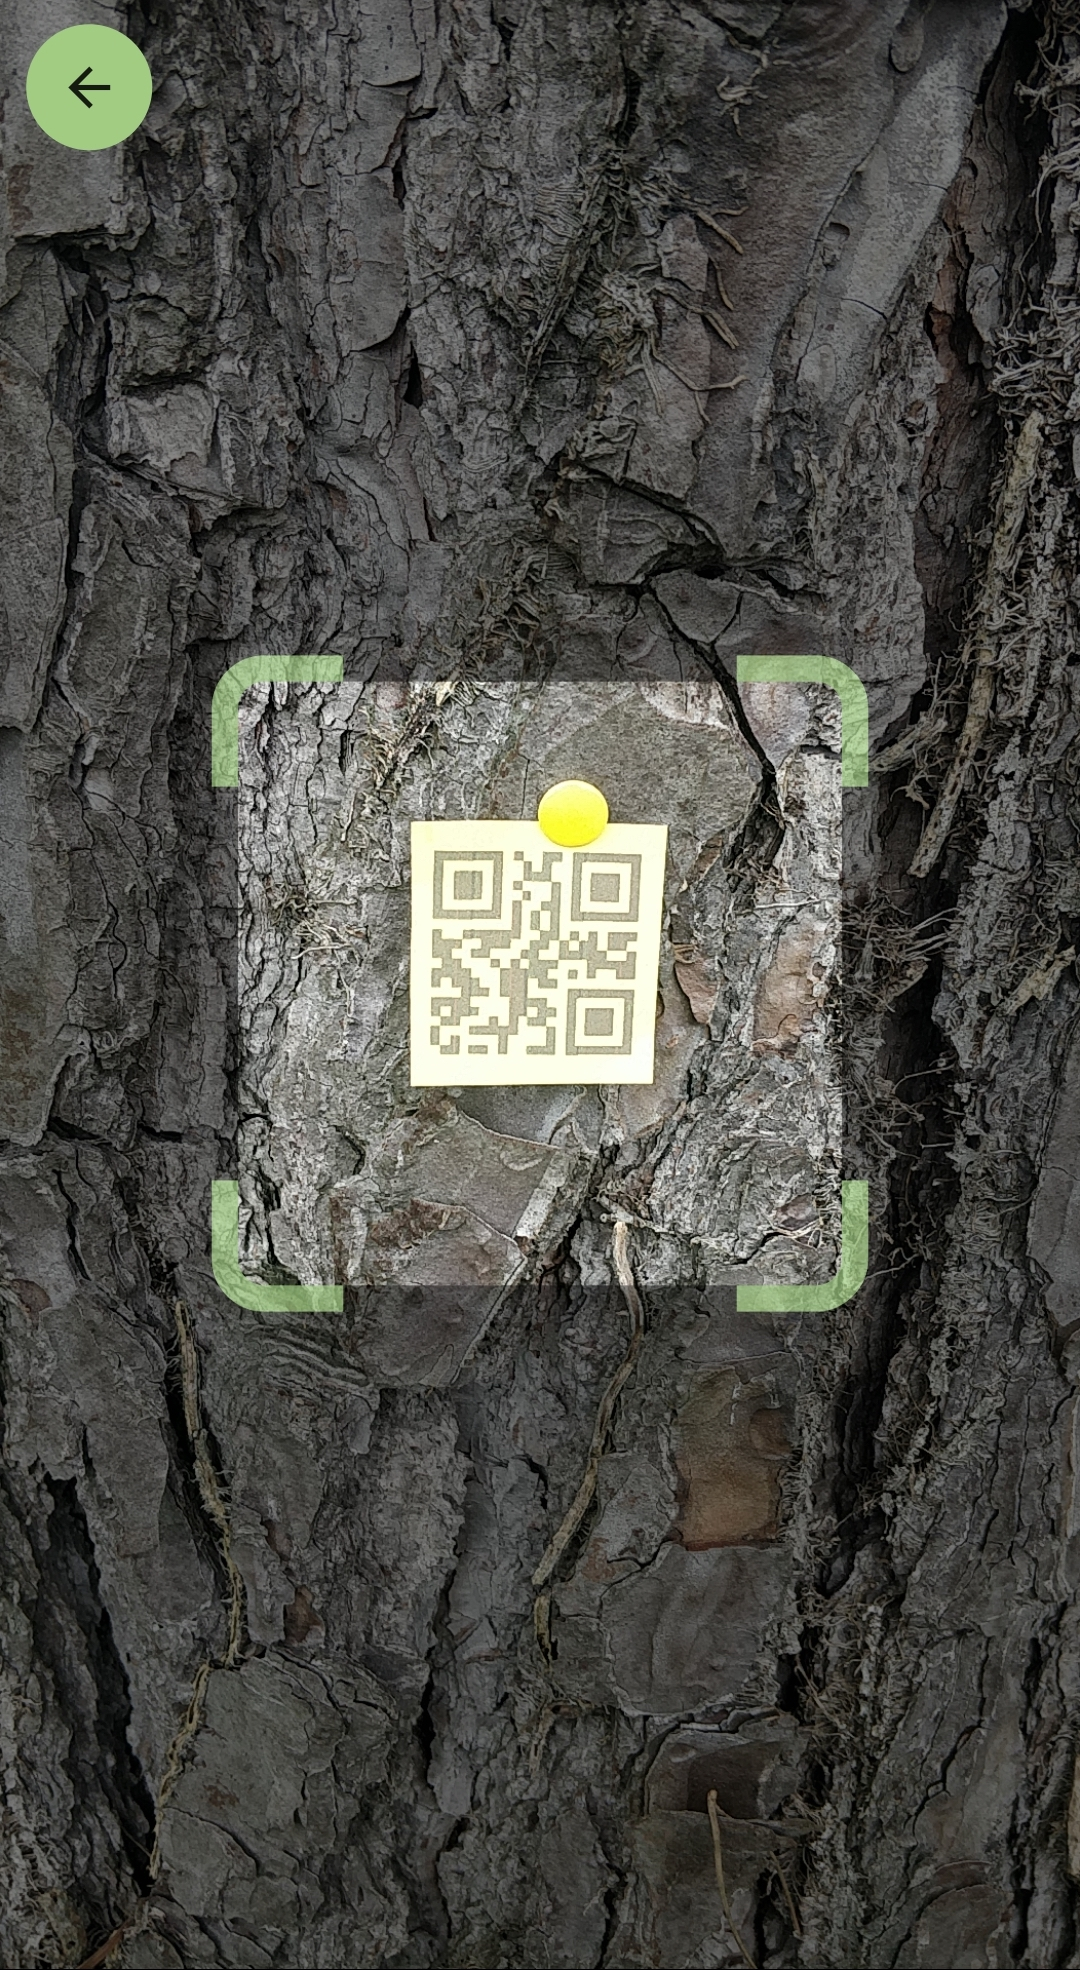
\includegraphics[width=0.30\textwidth]{img/app/scan_qr_old.jpg}
        \label{fig:scanQRapp}
    }
    \subfloat[Taniche di benzina in AR]{
        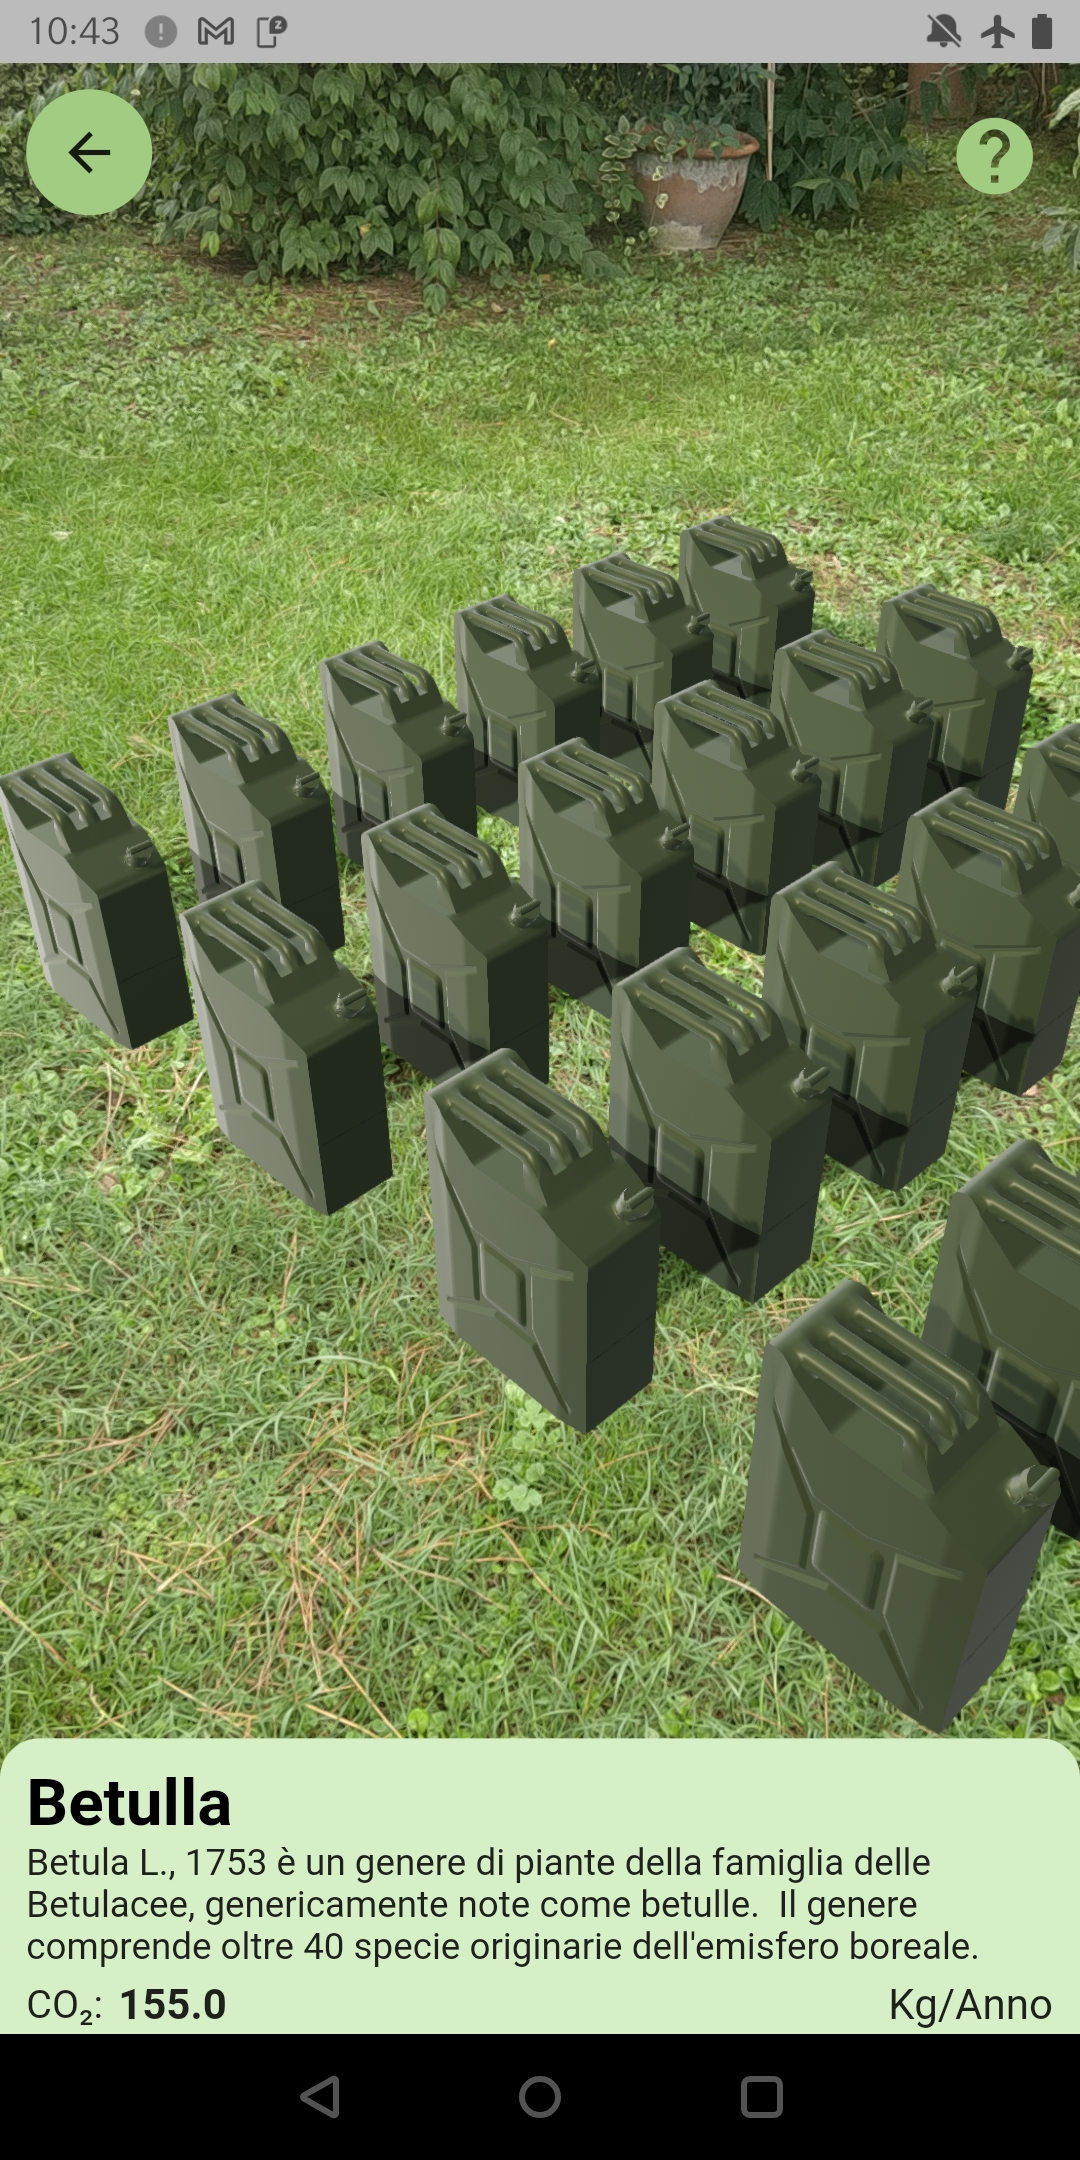
\includegraphics[width=0.30\textwidth]{img/app/ar_fuel.jpg}
        \label{fig:tankAR}
    }
    \subfloat[Plichi di carta in AR]{
        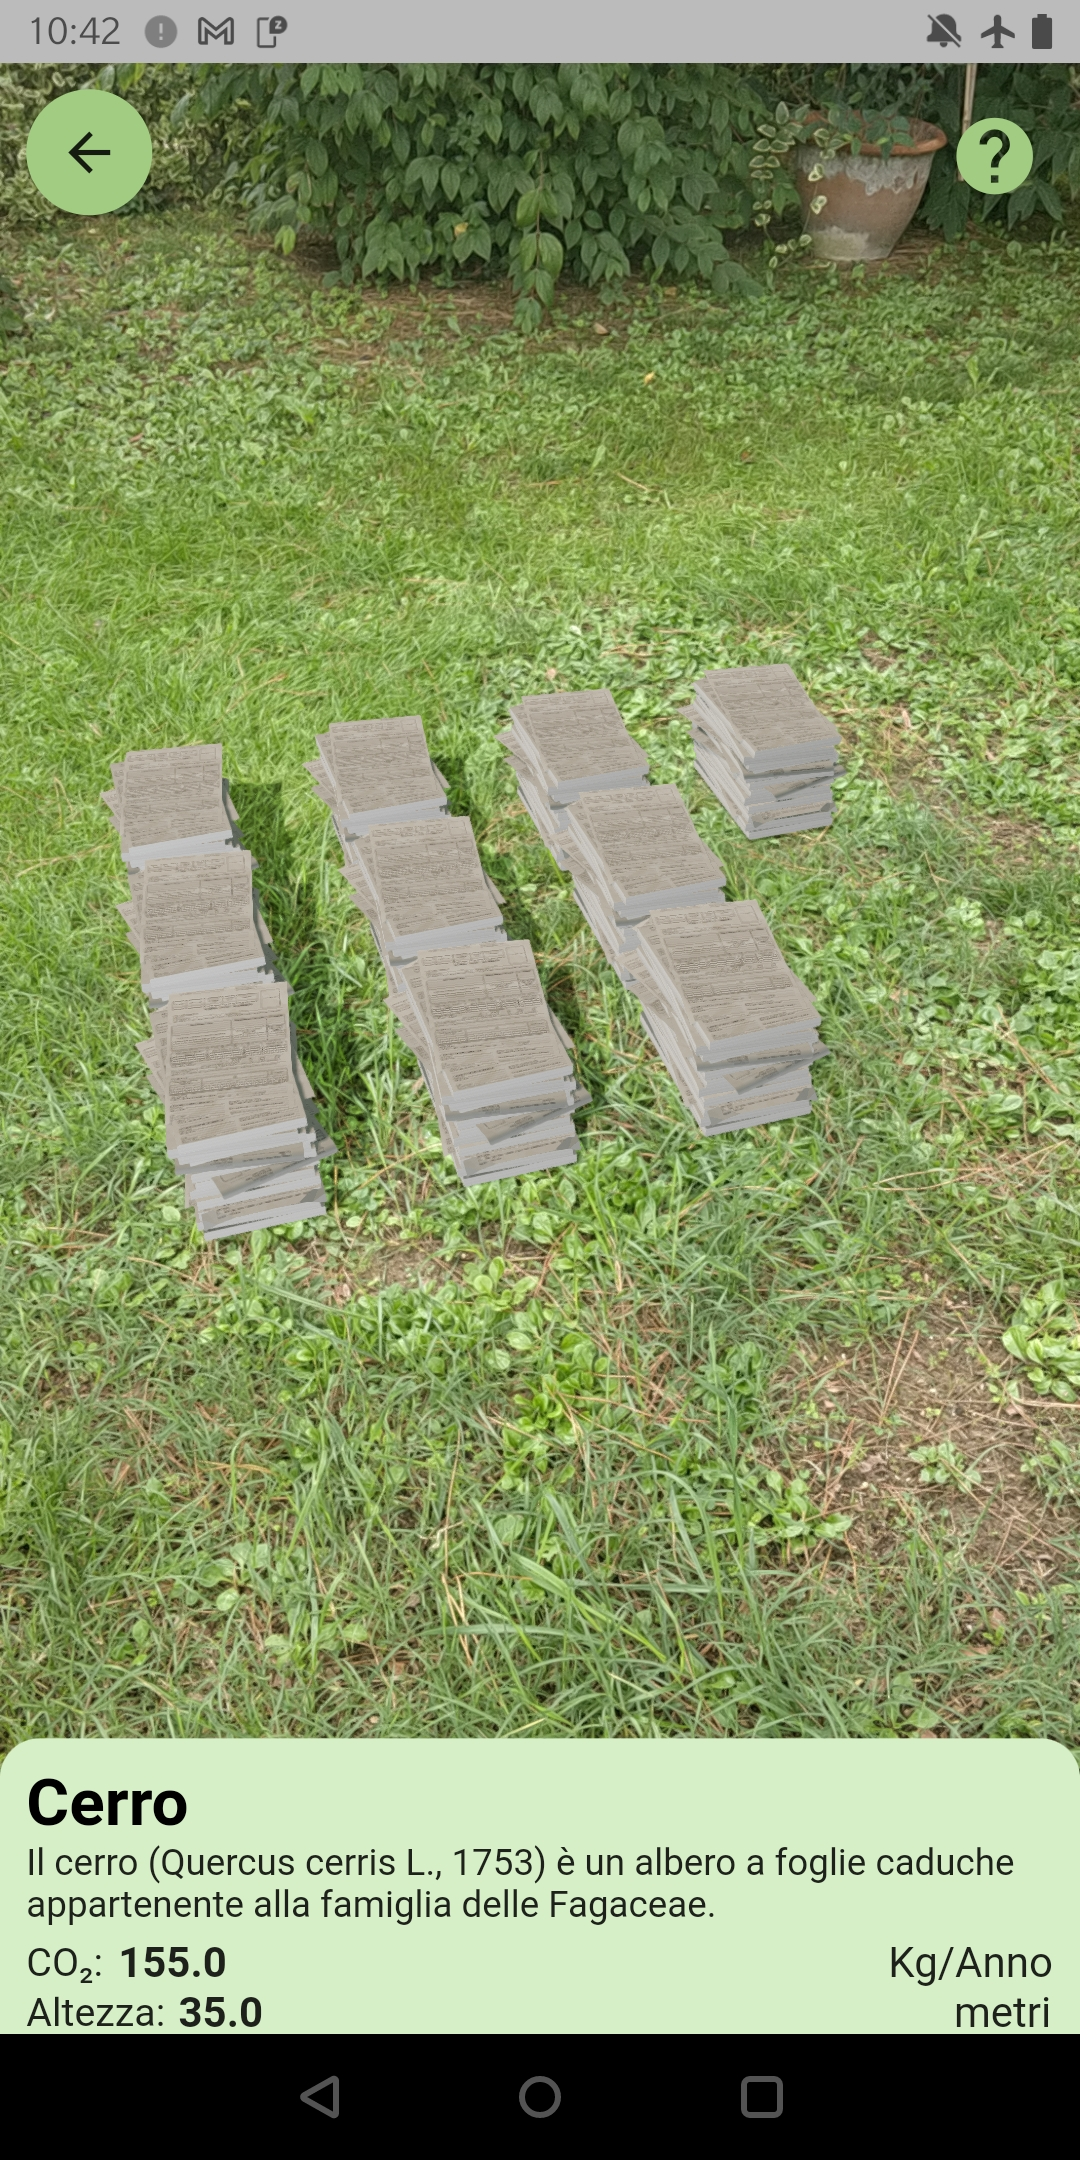
\includegraphics[width=0.30\textwidth]{img/app/ar_paper.jpg}
        \label{fig:paperAR}
    }
    \caption{Sessione AR dell'app mobile}
    \label{fig:arSession}
\end{figure}

Sono stati inseriti alcuni elementi della gamification (vedi sezione \ref{sec:gamification}), come i badge e i livelli, che mirano ad aumentare l'interesse e il coinvolgimento degli utenti.
Dopo la scansione di un albero, questo viene memorizzato nella collezione dell'utente che guadagna un badge aumentando di livello.
Tutti i progressi raggiunti e i risparmi virtualmente guadagnati vengono visualizzati all'interno della pagina personale (figura \ref{fig:userPage}) dove è possibile anche impostare i dati del profilo (es. nome, data di nascita e corso universitario) e una foto.

\begin{figure}
    \centering
    \subfloat[Profilo utente con progressi e badge acquisiti]{
        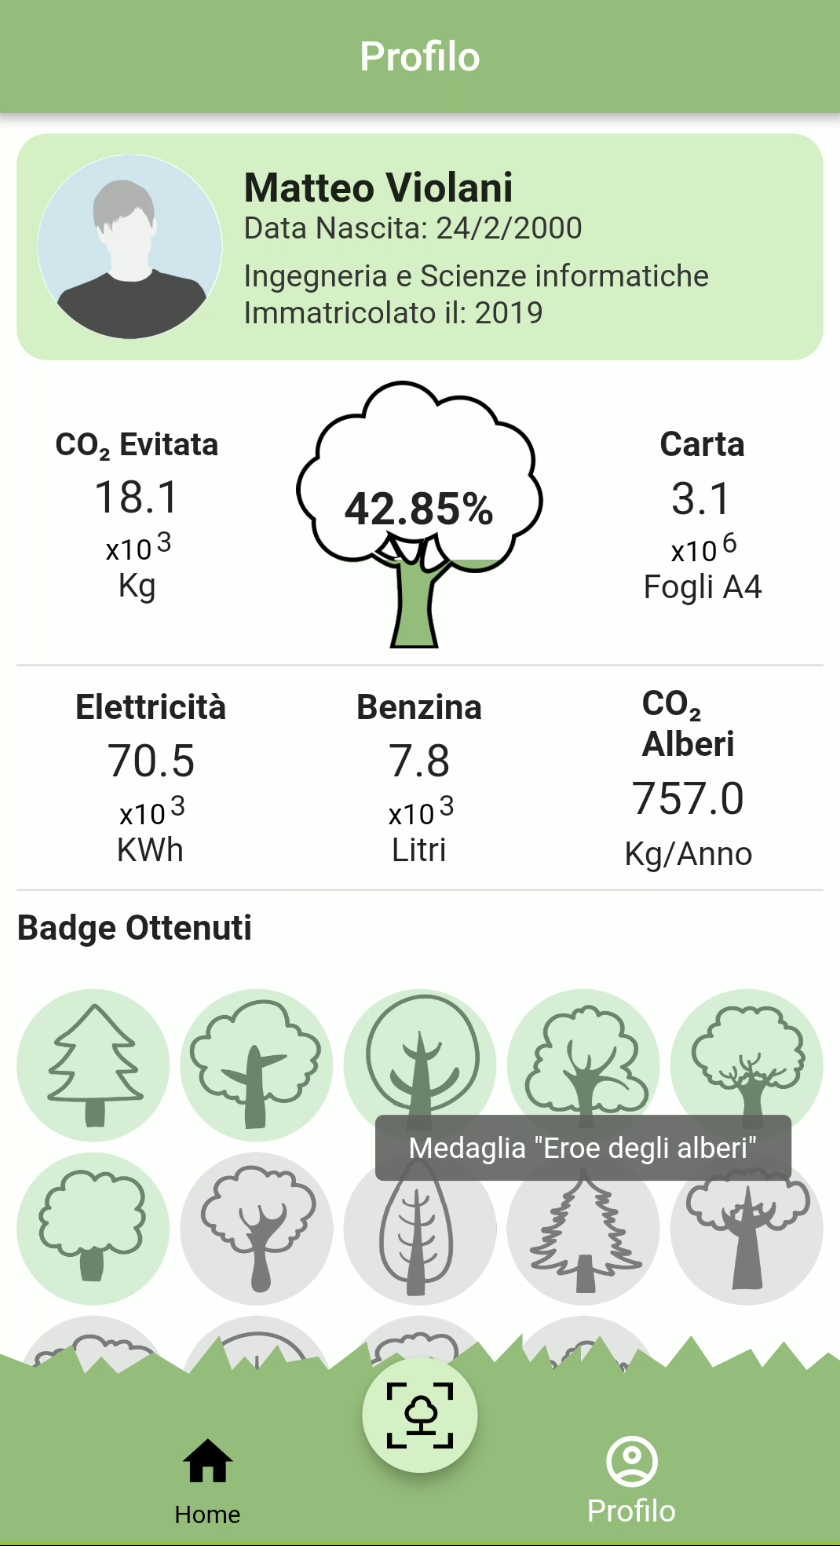
\includegraphics[width=0.30\textwidth]{img/app/user_page.png}
        \label{fig:userProgress}
    }
    \subfloat[Pagina di modifica dei dati utente]{
        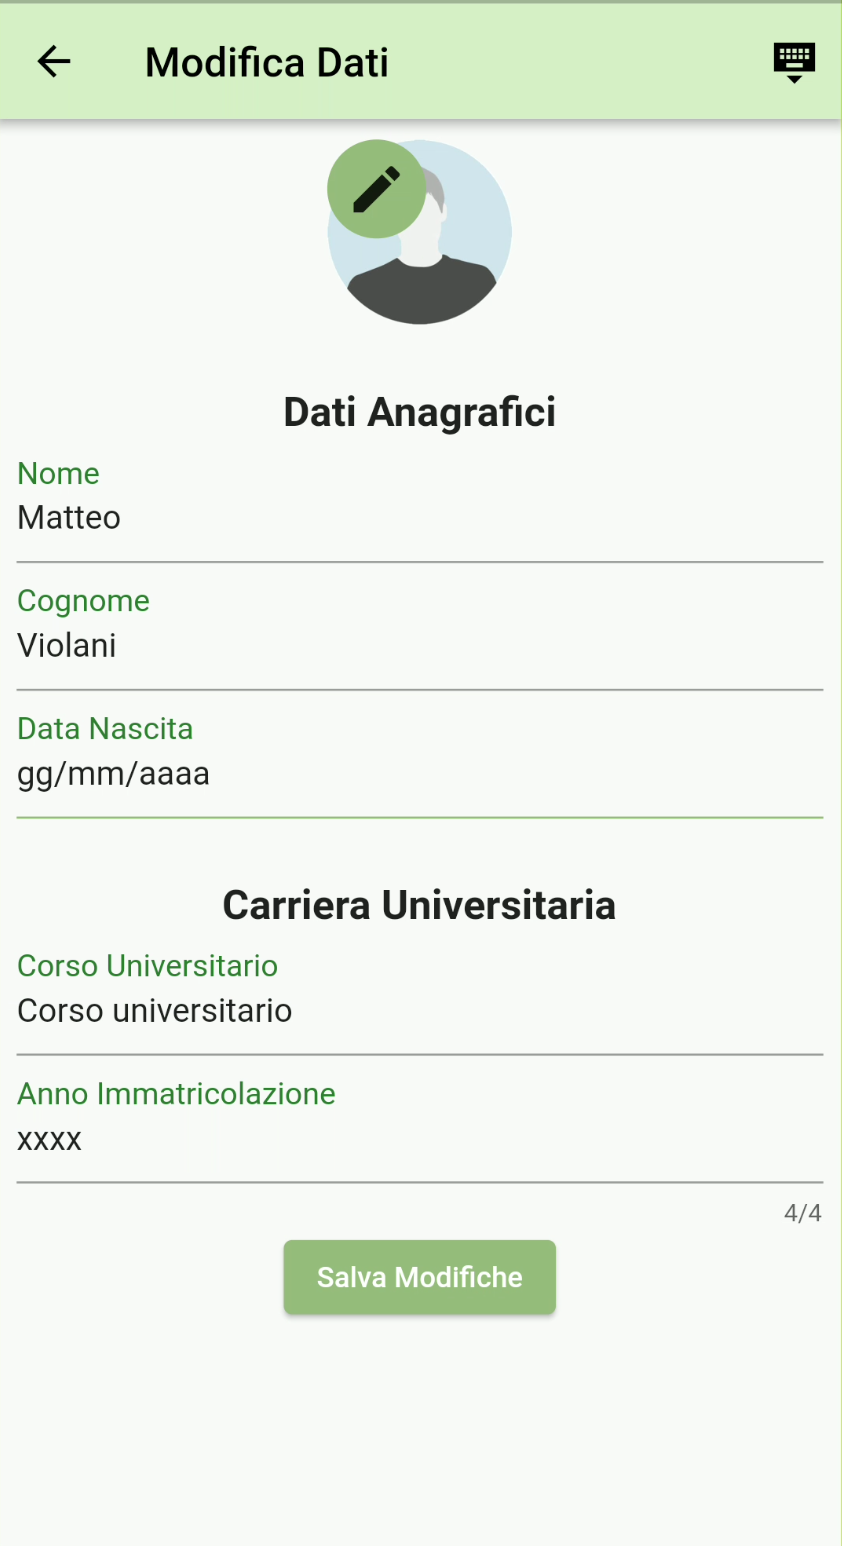
\includegraphics[width=0.30\textwidth]{img/app/edit_user.png}
        \label{fig:editUser}
    }
    \caption{Pagina utente app mobile}
    \label{fig:userPage}
\end{figure}

Gli alberi collezionati si trovano nella pagina principale (figura \ref{fig:treeHome}) con tutte le informazioni e la possibilità di avviare direttamente la sessione di realtà aumentata (figura \ref{fig:treeDetail}).
L'app è stata progettata per essere in grado di funzionare offline dopo una prima sincronizzazione necessaria con connessione ad internet.

\begin{figure}
    \centering
    \subfloat[Homepage alla prima installazione]{
        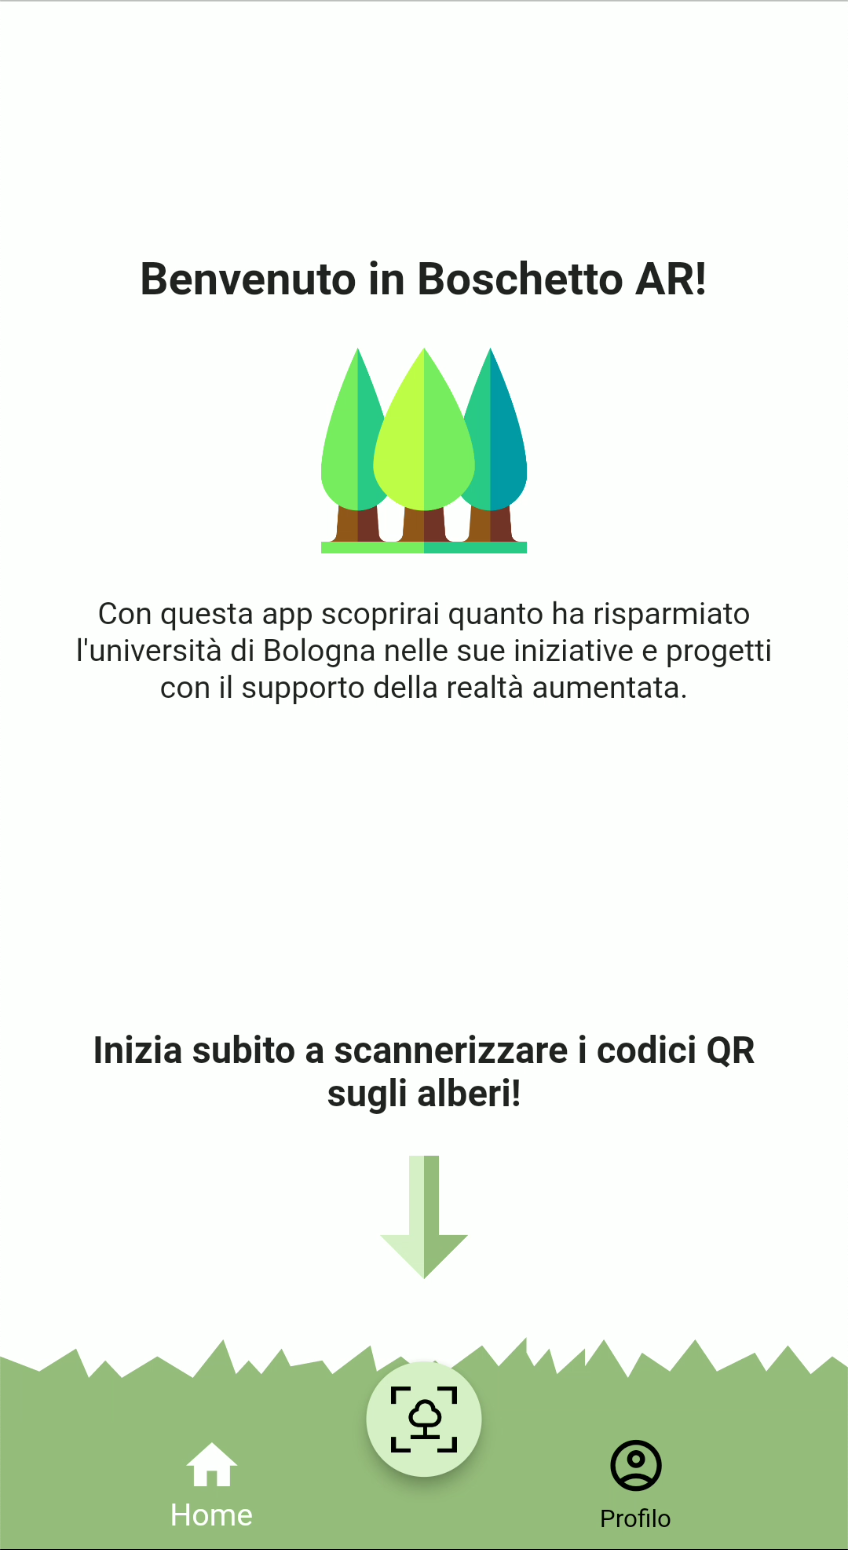
\includegraphics[width=0.30\textwidth]{img/app/first_launch.png}
        \label{fig:appFirstLaunch}
    }
    \subfloat[Collezione utente degli alberi scansionati]{
        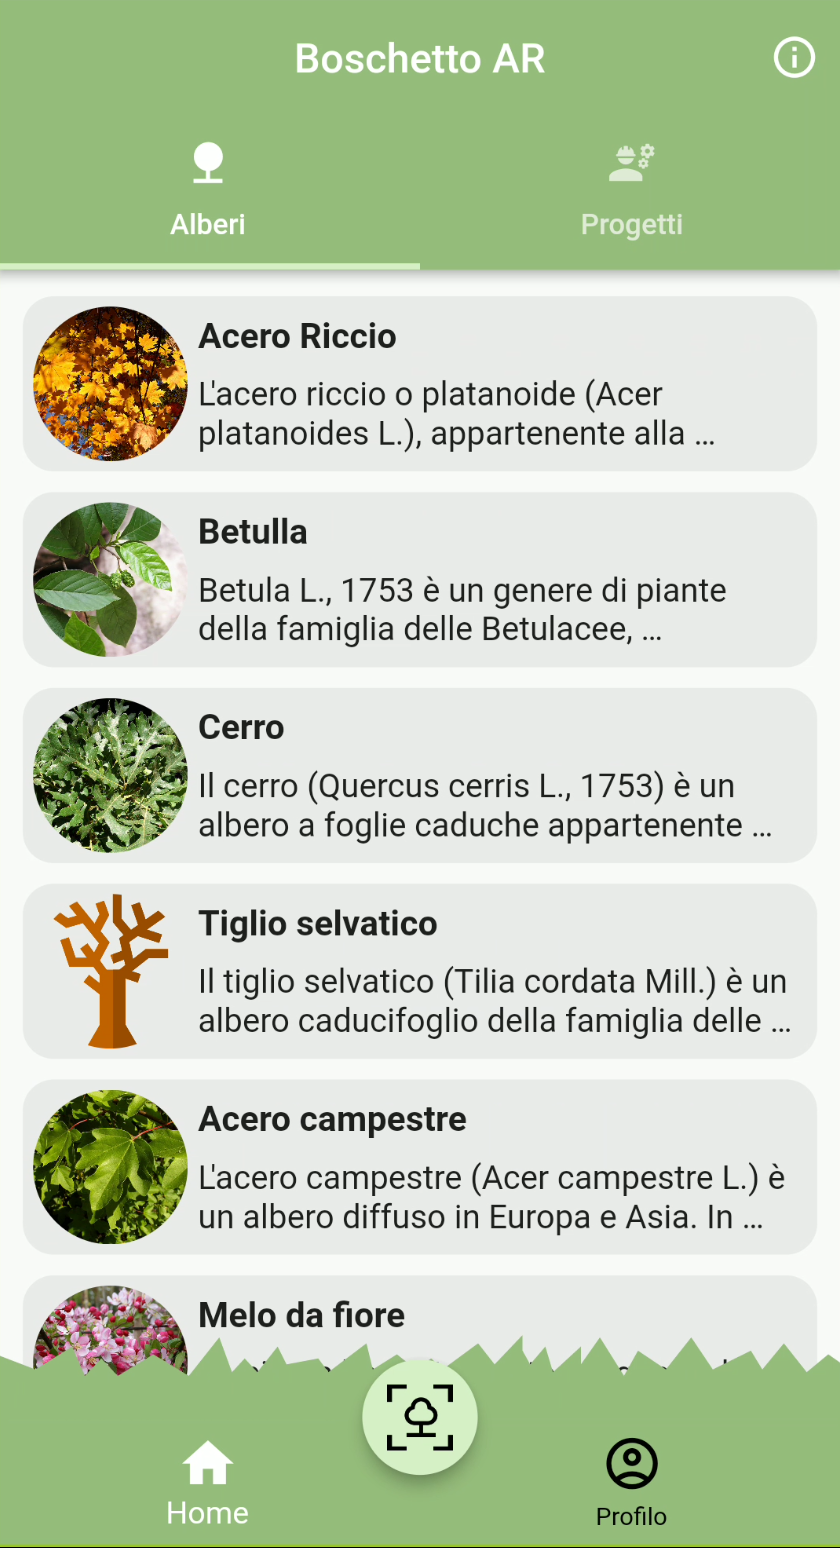
\includegraphics[width=0.30\textwidth]{img/app/treeHome.png}
        \label{fig:treeHome}
    }
    \subfloat[Pagina dei dettagli dell'albero con possibilità di avviare l'AR]{
        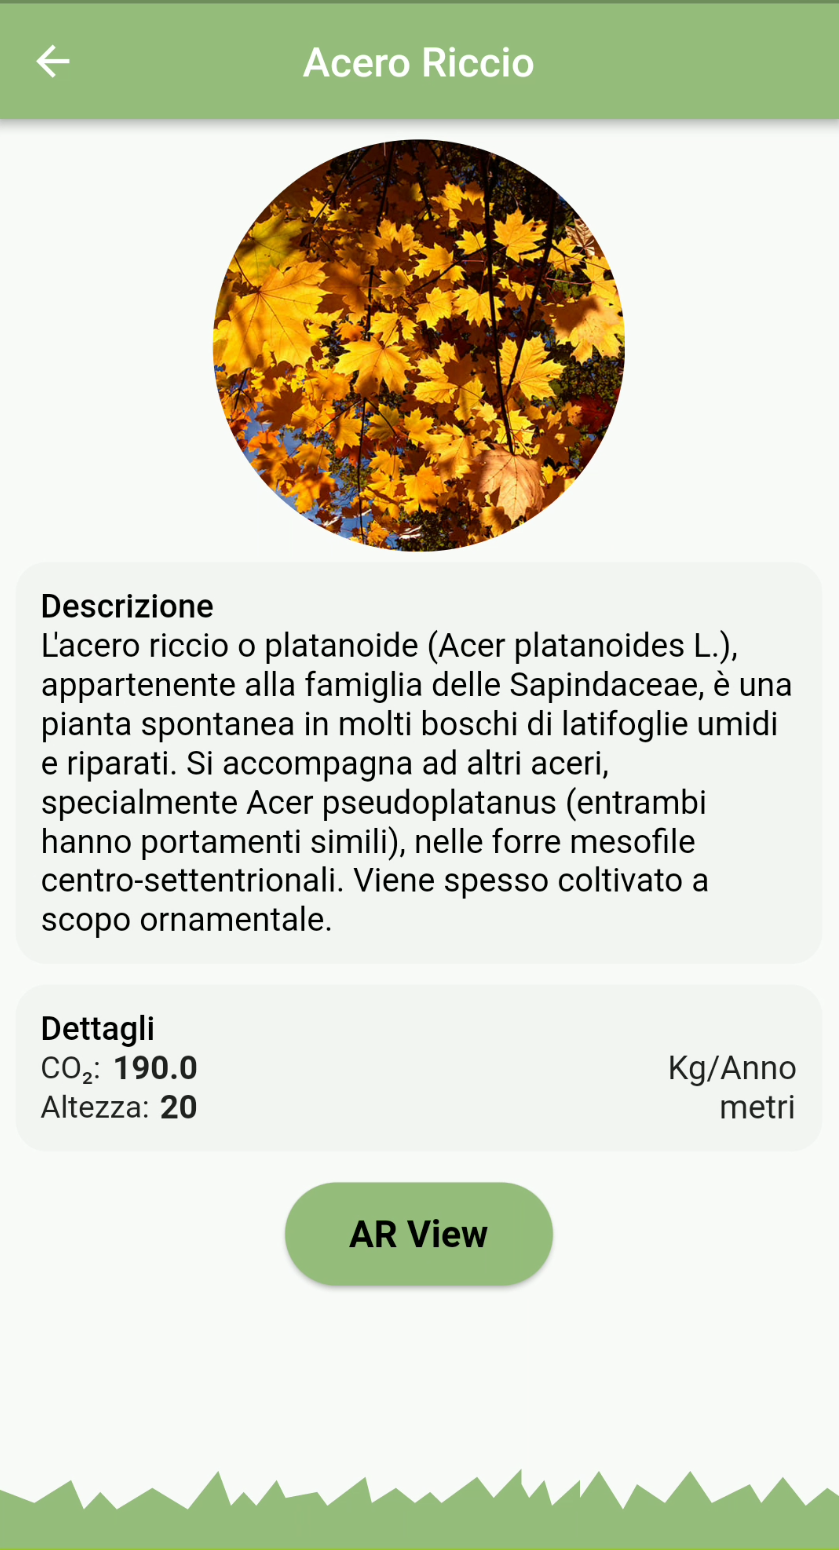
\includegraphics[width=0.30\textwidth]{img/app/treeDetailsOld.png}
        \label{fig:treeDetail}
    }
    \caption[Homepage app BoschettoAR]{Homepage app BoschettoAR e pagina con dettagli albero}
    \label{fig:homeApp}
\end{figure}

\subsection{Obiettivo}
L'obiettivo di questa tesi è di estendere l'esperienza fornita dall'app BoschettoAR integrando un totem interattivo che mostri il livello di consapevolezza raggiunta dalla comunità UniBo sul tema dell'inquinamento, attraverso la visualizzazione degli alberi collezionati (es. bosco virtuale) dagli utenti che hanno deciso di condividere i propri progressi raggiunti nell'app.

\section{Requisiti e analisi}
In questa sezione vengono elencati i requisiti funzionali e non che devono essere soddisfatti e raggiunti durante lo sviluppo dell'applicativo del totem e nell'aggiornamento dell'applicazione.
\subsection{Requisiti funzionali}
\subsubsection{App mobile}
\begin{itemize}
    \item Condivisone dei progressi: l'utente, dopo aver impostato un nickname, dovrà poter condividere i propri progressi raggiunti con il totem attraverso una schermata dedicata. Entro un certo intervallo di tempo il caricamento deve interrompersi automaticamente.
    \item La pagina per il caricamento dei progressi deve fornire una breve guida e indicare le informazioni che verranno condivise.
    \item Nella pagina dei dettagli di un albero collezionato deve essere mostrato anche il progetto associato e viceversa.
\end{itemize}
\subsubsection{Totem}
\begin{itemize}
    \item Devono essere presenti le schermate: homepage, statistiche, classifica e informazioni.
    \item La homepage deve mostrare gli utenti coinvolti e i dettagli dei loro progressi 
    \item La schermata delle statistiche deve mostrare il conteggio totale di alberi e progetti coinvolti, la carta, l'elettricità, la benzina, la corrente elettrica e la CO2 virtualmente risparmiate con la partecipazione degli utenti. Si deve mostrare una breve descrizione per ciascun dato mostrato.
    \item La classifica deve mostrare i 10 migliori utenti sulla base della co2 risparmiata.
    \item Nella pagina delle informazioni deve essere presente la spiegazione dei calcoli effettuati e una sezione con maggiori dettagli sul progetto ReMade. Deve essere possibile aggiungere nuove sezioni.
    \item Ricezione dei progressi: il totem deve ricevere i progressi dell'utente condivisi tramite app.
\end{itemize}
\subsection{Requisiti non funzionali}
\subsubsection{App mobile}
\begin{itemize}
    \item Il caricamento dei progressi non deve impiegare più 8 secondi altrimenti deve essere interrotto. A fine processo, anche in caso di errore, deve essere mostrata una schermata che informi l'utente con l'esito del caricamento dei dati.
\end{itemize}
\subsubsection{Totem}
\begin{itemize}
    \item L'utente deve poter depositare i progressi raggiunti in app in qualsiasi momento indipendentemente dalla schermata selezionata del totem. Deve quindi essere sempre accessibile il codice QR che identifica il totem in modo da poterlo scansionare tramite app.
    \item Il sistema deve essere scalabile in modo da permettere l'aggiunta di nuovi totem interattivi e gestire simultaneamente più richieste di condivisione dei dati dall'applicazione.
    \item L'interfaccia deve apparire familiare rispetto all'app mobile in modo da permettere un utilizzo immediato e non scoraggiare gli utenti all'interazione. Devono essere necessari un paio di tocchi per navigare tra le schermate e mostrare il codice QR.
    \item La sincronizzazione dei dati deve essere, per quanto possibile, immediata in modo da mostrare sempre dati aggiornati in tempo reale.
\end{itemize}
%
%
%
%
\section{Design}
\subsection{Modello del dominio}
I dati del totem, che vengono memorizzati all'interno del database nel cloud, riguardano le informazioni sul totem stesso (ad esempio il nome e la sede UniBo in cui si trova) e tutti i progressi degli utenti caricati tramite app.
Si ha quindi un'entità che rappresenta i progressi caricati dall'utente (\texttt{SharedData}) e un'entità che rappresenta il totem (\texttt{Totem}).
\begin{figure}[h!]
    \centering
    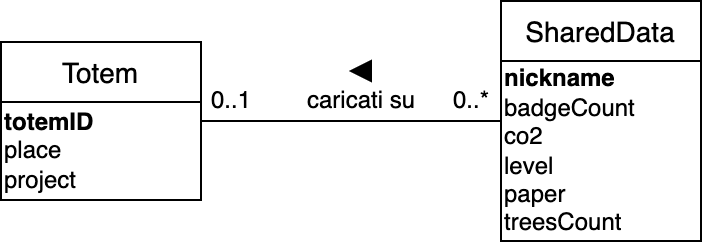
\includegraphics[width=0.5\textwidth]{img/totem/totemDomain.png}
    \caption[Modello del dominio del totem]{Modello del dominio del totem: in grassetto sono evidenziate le chiavi delle entità}
    \label{fig:totemDomain}
\end{figure}
\subsection{Architettura e pattern}
Il sistema si compone di tre componenti principali: l'app mobile, il totem e il cloud database. I progressi dell'utente dall'app vengono caricati sul database quindi scaricati nel totem. In figura \ref{fig:communication-schema} viene mostrato lo schema delle interazioni fra i tre componenti del sistema durante la condivisione dei progressi.
Il database fornisce inoltre le informazioni sugli alberi e i relativi progetti sia al totem che all'app mobile.
\begin{figure} [h]
    \centering
    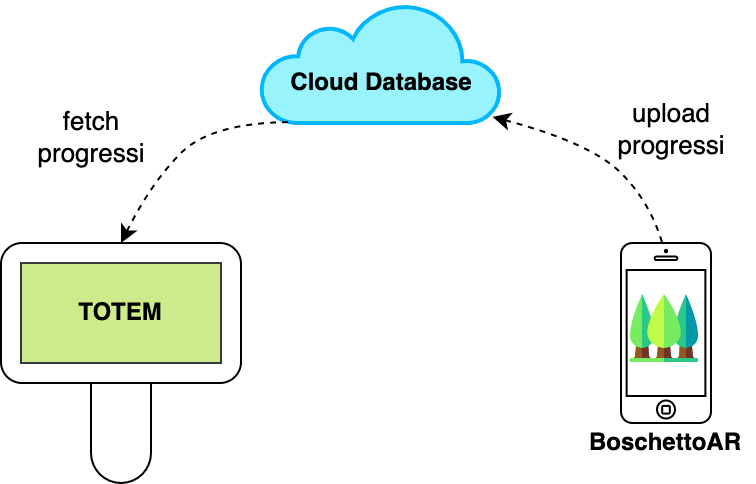
\includegraphics[width=0.6\textwidth]{img/totem/arch-totem-app-dati.png}
    \caption{Schema della architettura e interazione fra app e totem}
    \label{fig:communication-schema}
\end{figure}

Per quanto riguarda l'architettura del software del totem, come per l'app mobile, viene utilizzata una forma del pattern architetturale MVI (\textit{Model-View-Intent}).
\begin{itemize}
    \item La \textbf{View} è responsabile dell'interfaccia grafica e della visualizzazione dei dati ricevuti dal \textit{Model}. A ogni evento, generato dall'interazione dell'utente, la View reagisce e comunica con il Model attraverso gli \textit{Intent}s.
    \item Il \textbf{Model} rappresenta lo stato dell'applicazione e contiene dati e informazioni. Fornisce un'interfaccia che espone metodi che rappresentano gli \textit{Intent}s innescabili dalla \textit{View} e che restituiscono un nuovo \textit{State}.
    \item Gli \textbf{Intent} sono eventi, generati dalla \textit{View}, che possono innescare una richiesta o modifica dei dati del \textit{Model}.
    \item Lo \textbf{State} viene creato dal \textit{Model} e viene inviato alla \textit{View} in risposta alle richieste avanzate dagli \textit{Intent}s. Lo State è una struttura dati immutabile che contiene i dati aggiornati del \textit{Model} o uno stato di una certa operazione (es. caricamento d'informazioni sul cloud) che devono essere visualizzati nella \textit{View}.
\end{itemize}
\begin{figure}[h!]
    \centering
    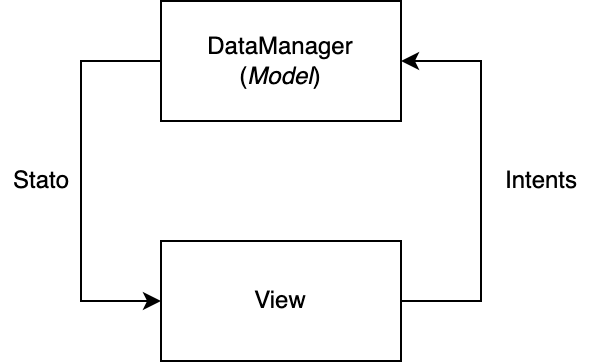
\includegraphics[width=0.55\textwidth]{img/totem/mvi-schema.png}
    \caption[Schema pattern MVI]{Schema pattern MVI: gli eventi della View vengono comunicati al Model che risponde con uno State con dati aggiornati da visualizzare.}
    \label{fig:mviPattern}
\end{figure}

% Per esempio nell'app mobile, dopo la scansione del codice QR di un albero, viene generato dalla \textit{View} un \textit{Intent} per aggiungere il nuovo albero. Il \textit{Model} effettua la modifica ai dati persistenti e risponde con un flusso di stati contenenti informazioni sullo'esito dell'operazione in tempo reale che viene visualizzato nella \textit{View} (es. schermata di caricamento).

Per l'accesso ai dati si è fatto uso del componente architetturale \textit{Repository} \cite{repositoryComponent} (figura \ref{fig:repository}) che è un'interfaccia, o classe astratta, che fornisce un unico punto di accesso ai dati, provenienti da diversi \textit{Provider}, incapsulandone l'elaborazione e la gestione. I \textit{Provider} sono componenti che forniscono l'accesso a una determinata risorsa dati come può essere un servizio web o un database.
\begin{figure}[h]
    \centering
    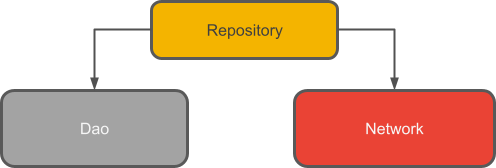
\includegraphics[width=0.55\textwidth]{img/repository.png}
    \caption{Componente repository con riferimenti a Dao e Network \cite{repositoryComponent}}
    \label{fig:repository}
\end{figure}
Nel caso del totem si ha solo \texttt{FirebaseProvider}, per accedere ai dati nel cloud, mentre nell'app mobile sono presenti anche \texttt{DatabaseProvider} e \texttt{PreferenciesProvider} (figura \ref{fig:repositorySchemaAPP}) che forniscono l'accesso ai dati persistenti memorizzati sullo smartphone. Per entrambe i dispositivi la classe che funge da \textit{Repository} è \texttt{DataMnager}.
Il repository comunica con i provider attraverso un'interfaccia DAO (\textit{Data Access Object}) specifica per ciascuno di questi e permette di definire le operazioni eseguibili nascondendo l'aspetto implementativo (es. query SQL).
\begin{figure}[h]
    \centering
    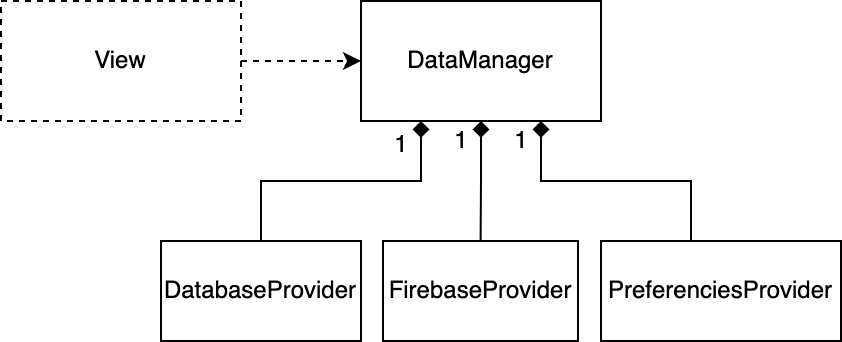
\includegraphics[width=0.7\textwidth]{img/app/repository_pattern_scheme.png}
    \caption{Schema UML architettura accesso ai dati, nell'app mobile, con componente Repository: l'interfaccia \texttt{DataManager} è il Repository, mentre \texttt{DatabaseProvider}, \texttt{FirebaseProvider} e \texttt{PreferenciesProvider} sono le interfacce dei singoli fornitori e sorgenti di dati (\textit{Providers}).}
    \label{fig:repositorySchemaAPP}
\end{figure}
\newpage
\subsection{Mockup}
Attraverso i \textit{mockup}, vengono presentate e spiegate le diverse schermate del totem.
Il termine \textit{mockup} o \textit{mock-up}, in italiano \enquote*{modello}, è una realizzazione a scopo illustrativo o espositivo di un oggetto o sistema, senza le complete funzioni dell'originale. Viene tipicamente sviluppato per fornire un'idea visiva del prodotto finale ai clienti, permettendo di effettuare correzioni o modifiche sulla bozza del prodotto ancora prima che si passi alla fase di sviluppo.

\subsubsection{Mobile app}
La pagina per la condivisione dei dati, mostrata in figura \ref{fig:sharePage}, fornisce all'utente una breve spiegazione e informa quali dati verranno condivisi e mostrati pubblicamente nel totem.
Cliccando sul pulsante \enquote*{Procedi} si passa all'identificazione del totem tramite codice QR (figura \ref{fig:scanTotem}) e successivamente alla schermata di caricamento dei dati sul totem (figura \ref{fig:uploadinData}).
\begin{figure}[h!]
    \centering
    \subfloat[Pagina di condivisone progressi]{
        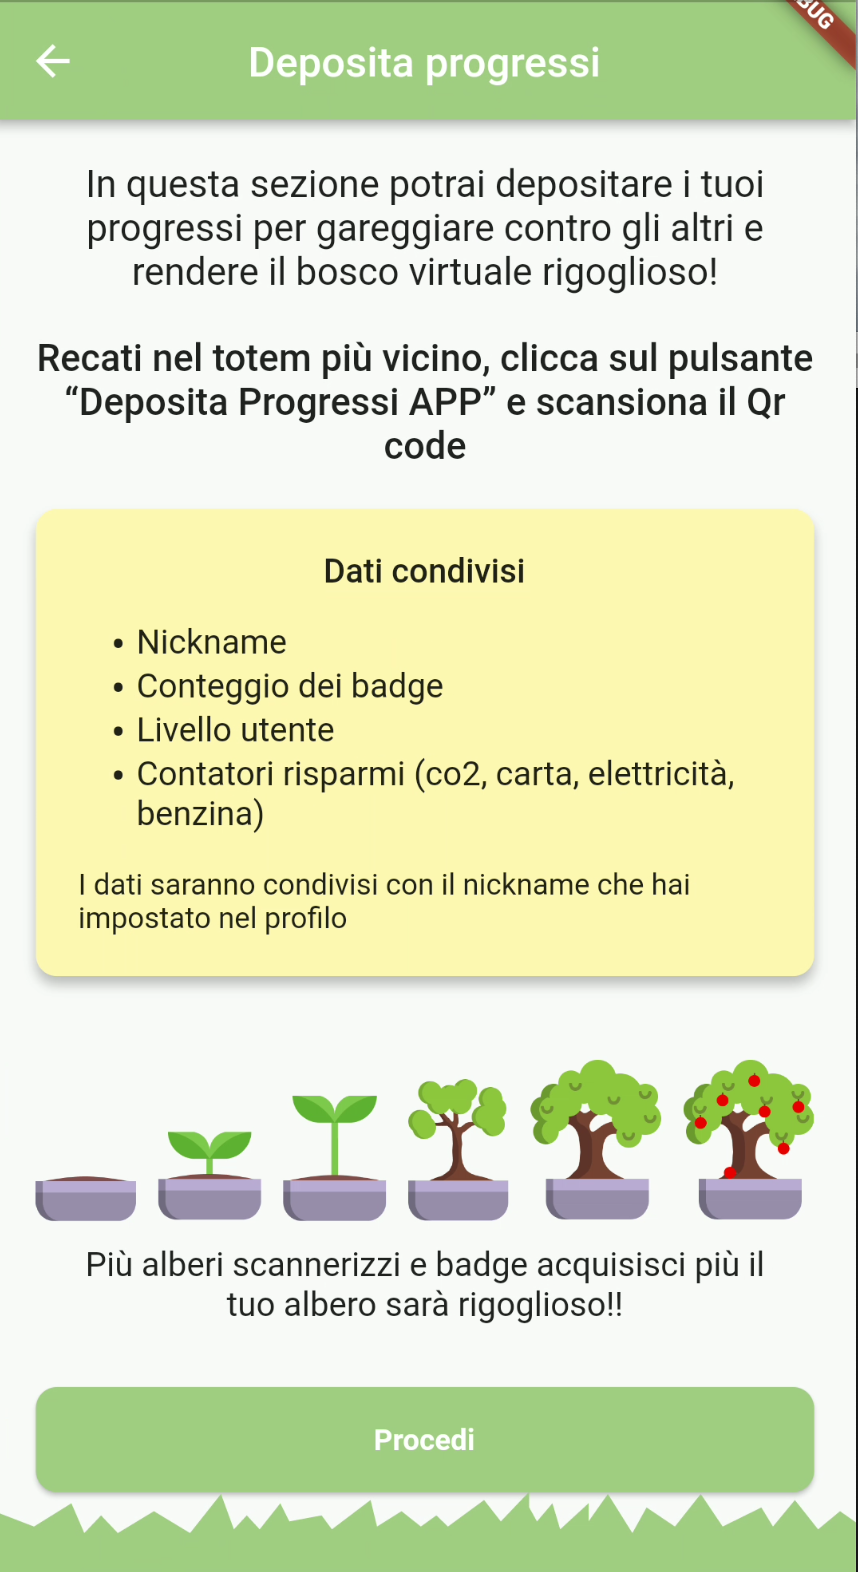
\includegraphics[width=0.3\textwidth]{img/app/uploadPage.png}
        \label{fig:sharePage}
    }
    \subfloat[Scansione QR code totem]{
        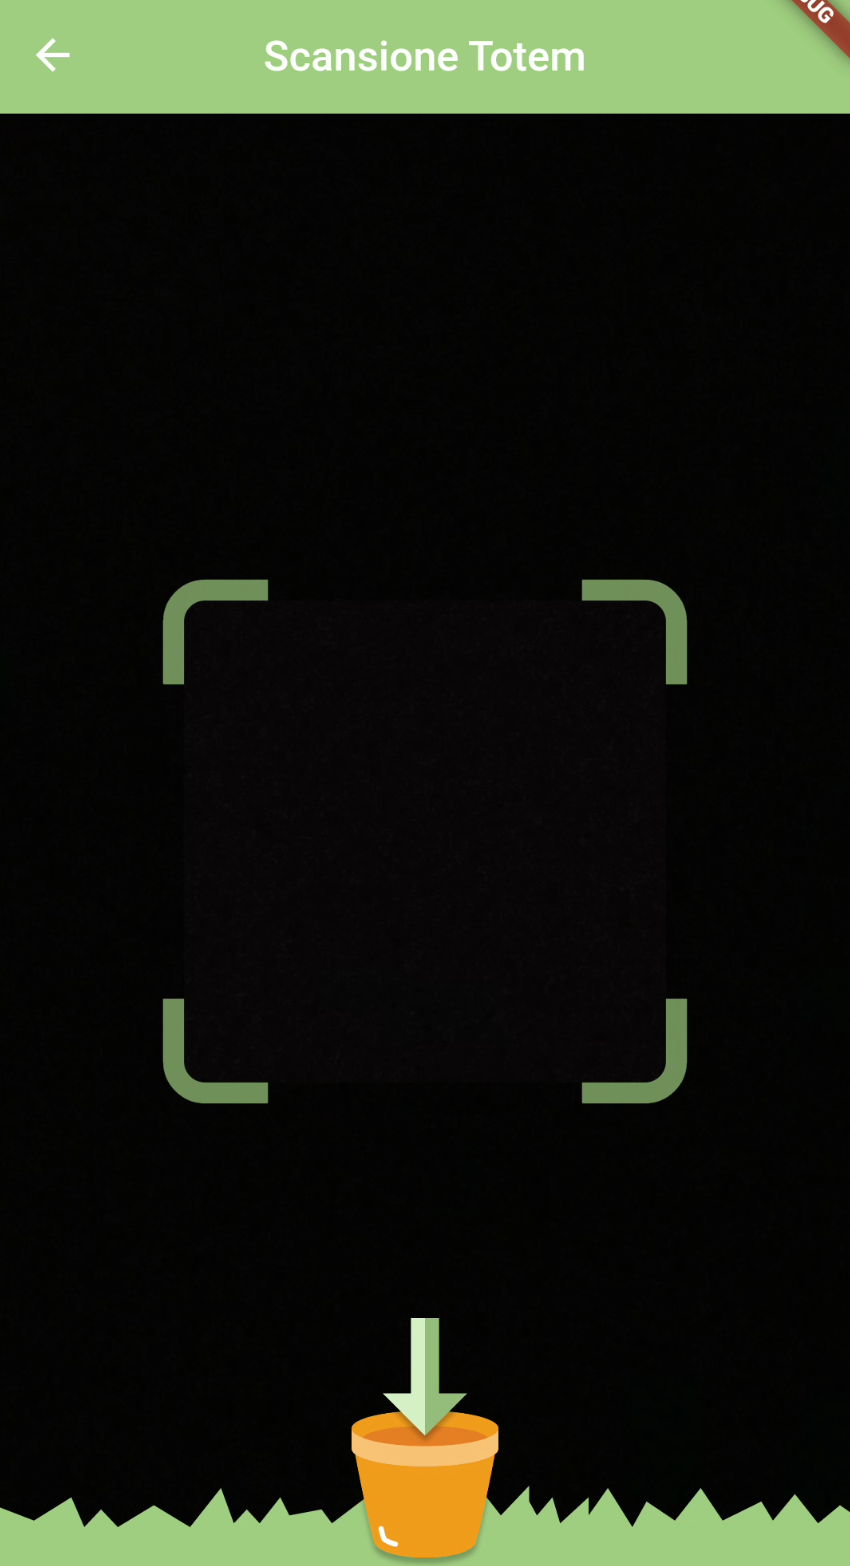
\includegraphics[width=0.3\textwidth]{img/app/uploadProgress.png}
        \label{fig:scanTotem}
    }
    \subfloat[Schermata di caricamento progressi]{
        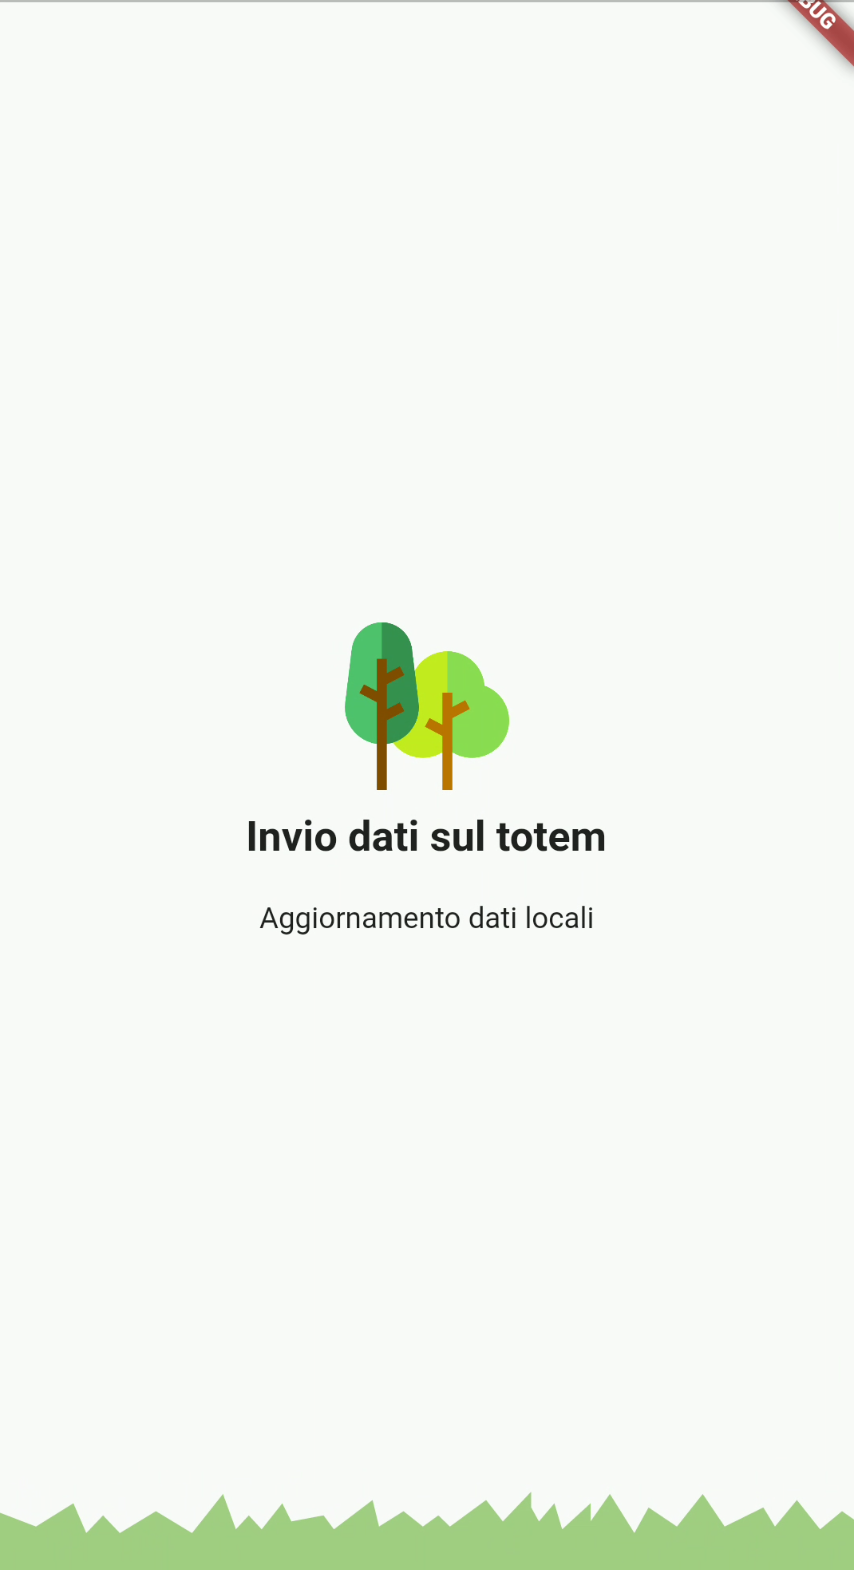
\includegraphics[width=0.3\textwidth]{img/app/uploadingPage.png}
        \label{fig:uploadinData}
    }
    \caption{Schermate condivisione dati da app}
    \label{fig:shareDataApp}
\end{figure}

\subsubsection{Totem}
La struttura dell'interfaccia del totem si suddivide in due sezioni principali: una colonna a sinistra contenente la barra di navigazione e la sezione con il QR code del totem e lo spazio restante a destra dove viene visualizzata la pagina selezionata (figura \ref{fig:viewStruct}).
\begin{figure}[h]
    \centering
    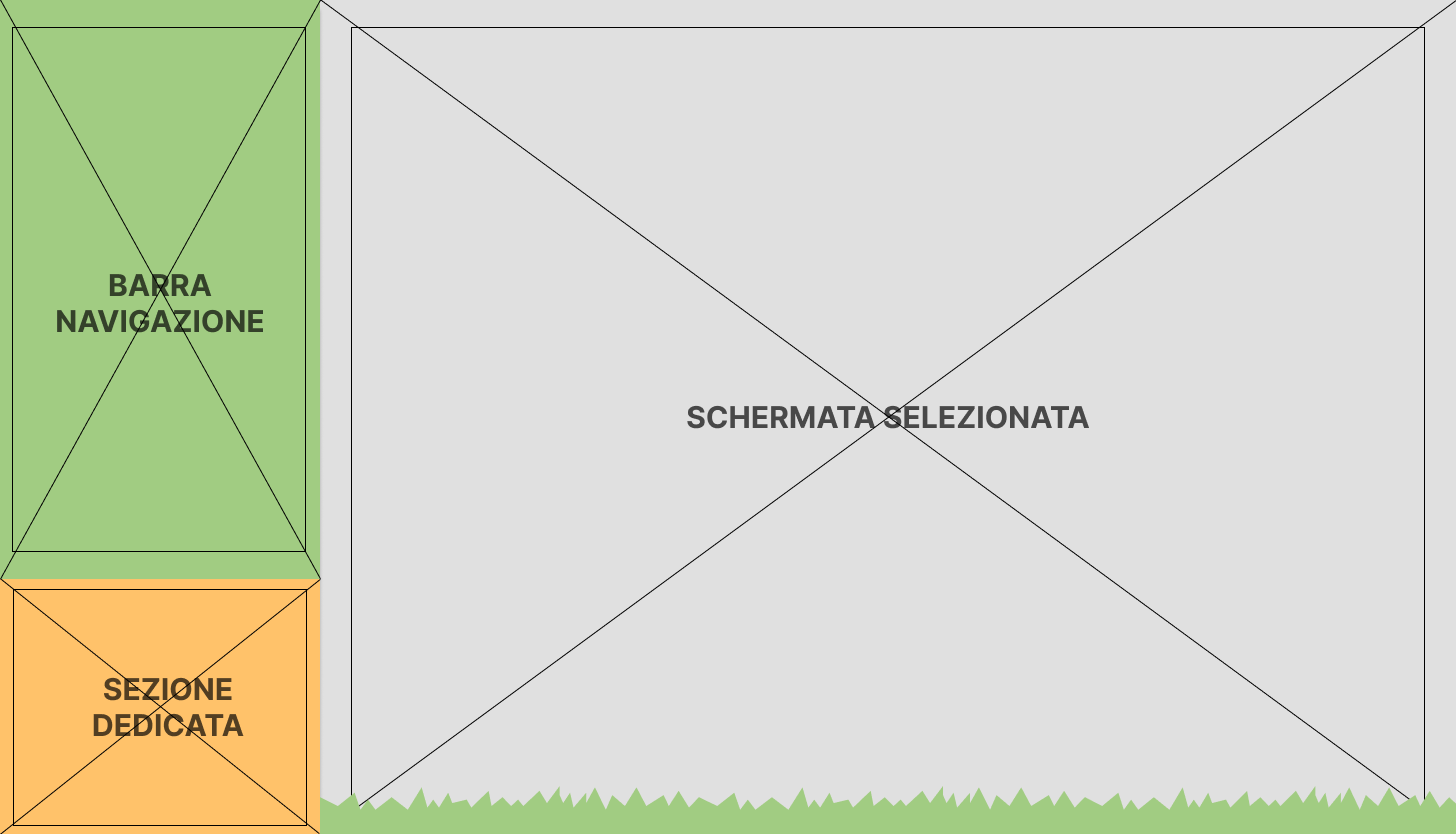
\includegraphics[width=0.8\textwidth]{img/totem/mainStructure.png}
    \caption{Layout generale della UI del totem}
    \label{fig:viewStruct}
\end{figure}

Vengono mantenuti i colori, il particolare dell'erba (figura \ref{fig:grassDetails}) e altre grafiche e icone, in modo da avere coerenza e continuità fra gli applicativi.
\begin{figure}[h]
    \centering
    
\includegraphics[width=0.4\textwidth]{img/totem/grassDetail.png}
    \caption{Dettaglio dell'erba presente nella'app e nel totem}
    \label{fig:grassDetails}
\end{figure}

In figura \ref{fig:depositIconsQR} viene mostrata l'icona del pulsante che mostra il codice QR del totem. Al tocco del pulsante, questo si ingrandisce rendendo visibile al suo interno il codice QR (figura \ref{fig:showQR}).
\begin{figure}
    \centering
    \subfloat[Codice QR del totem nascosto]{
        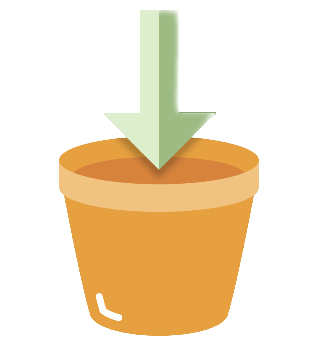
\includegraphics[width=2.5cm]{img/totem/depositIcon.png}
        \label{fig:hideQR}
    }
    \vspace{1cm}
    \subfloat[Codice QR del totem visibile]{
        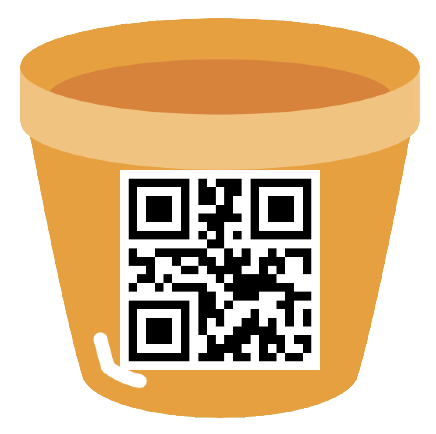
\includegraphics[width=2.5cm]{img/totem/depositQR.png}
        \label{fig:showQR}
    }
    \caption[Icone del QR code nel totem]{Icone del pulsante per mostrare il codice QR del totem e avviare la condivisione}
    \label{fig:depositIconsQR}
\end{figure}

Per quanto riguarda la homepage sono stati fatti due mockup con design differenti: nel primo vengono mostrati gli utenti come piccoli alberi disposti su delle mensole (figura \ref{fig:shelfHome}), nel secondo viene utilizzato un layout a griglia e gli utenti vengono rappresentati come chiome di alberi visti dall'alto (figura \ref{fig:forestHome}) ricreando un vero e proprio boschetto virtuale. In entrambi i casi il tocco di un elemento espande il pannello dei dettagli e le chiome degli alberi crescono al crescere del livello utente con lo scopo di stimolare ulteriormente la scansione di nuovi alberi e di conseguenza la consapevolezza sul tema del risparmio di carta e piantumazione di nuovi alberi.
\begin{figure}
    \centering
    \subfloat[Visualizzazione a mensole]{
        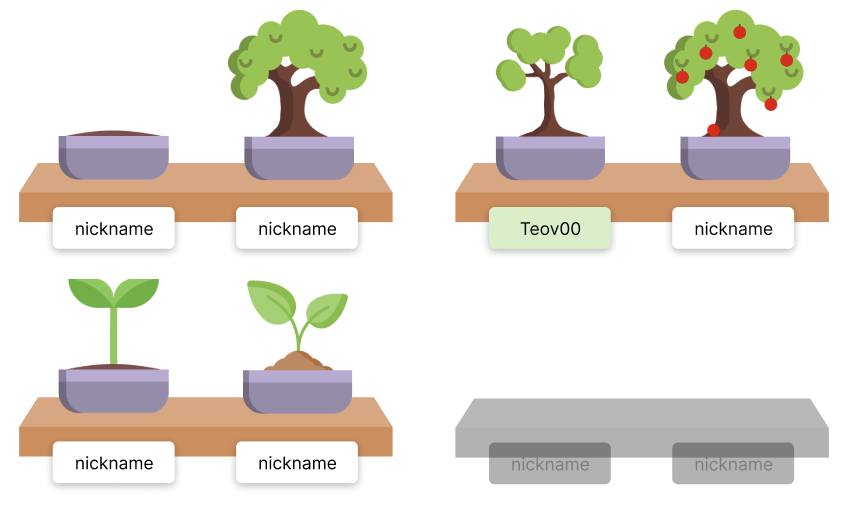
\includegraphics[width=0.45\textwidth]{img/totem/shelfViewHome.png}
        \label{fig:shelfHome}
    }
    \subfloat[Visualizzazione a bosco]{
        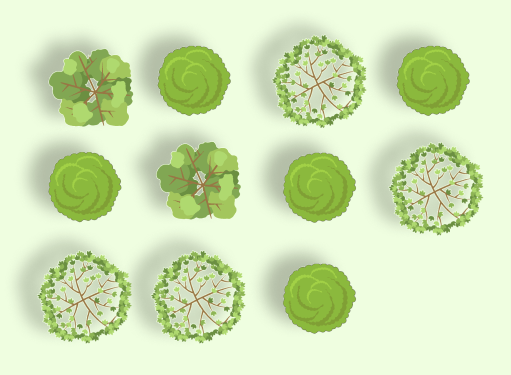
\includegraphics[width=0.4\textwidth]{img/totem/forestViewHome.png}
        \label{fig:forestHome}
    }
    \caption[Alternative di homepage nel totem]{Design alternativi per la homepage del totem}
    \label{fig:homepages}
\end{figure}

Il pannello dei dettagli utente si trova in alto a destra nella homepage e mostra il nickname, i progressi e il livello raggiunti dell'utente selezionato. Sono stati pensati tre diversi design  che differiscono per decorazione; si ha quindi la mensola, il cordino e lo stile tondeggiante (rispettivamente figura \ref{fig:shelfDetail}, \ref{fig:cordDetail}, \ref{fig:roundDetail}).

\begin{figure}
    \centering
    \subfloat[Stile mensola]{
        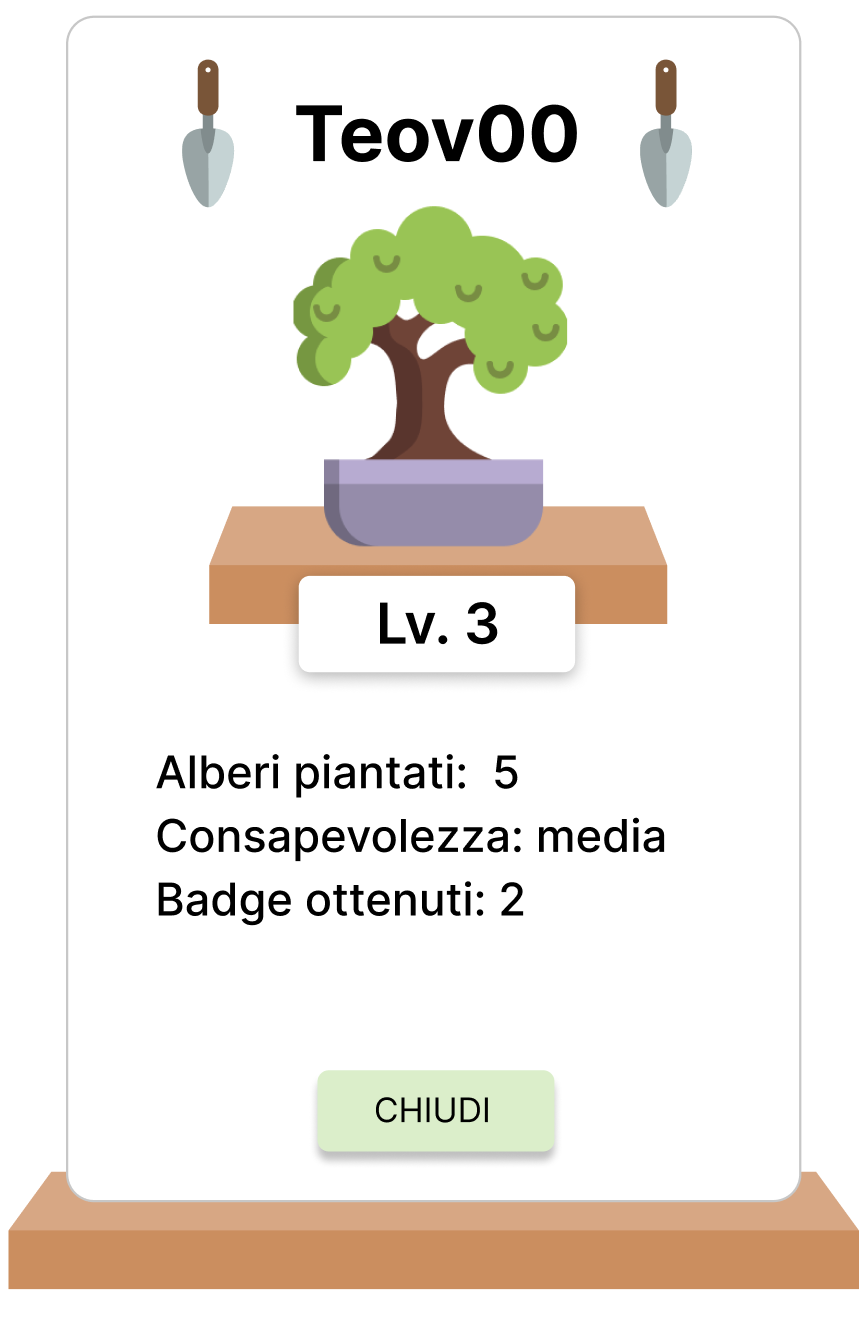
\includegraphics[width=0.30\textwidth]{img/totem/shelfDetail.png}
        \label{fig:shelfDetail}
    }
    \subfloat[Stile tendina]{
        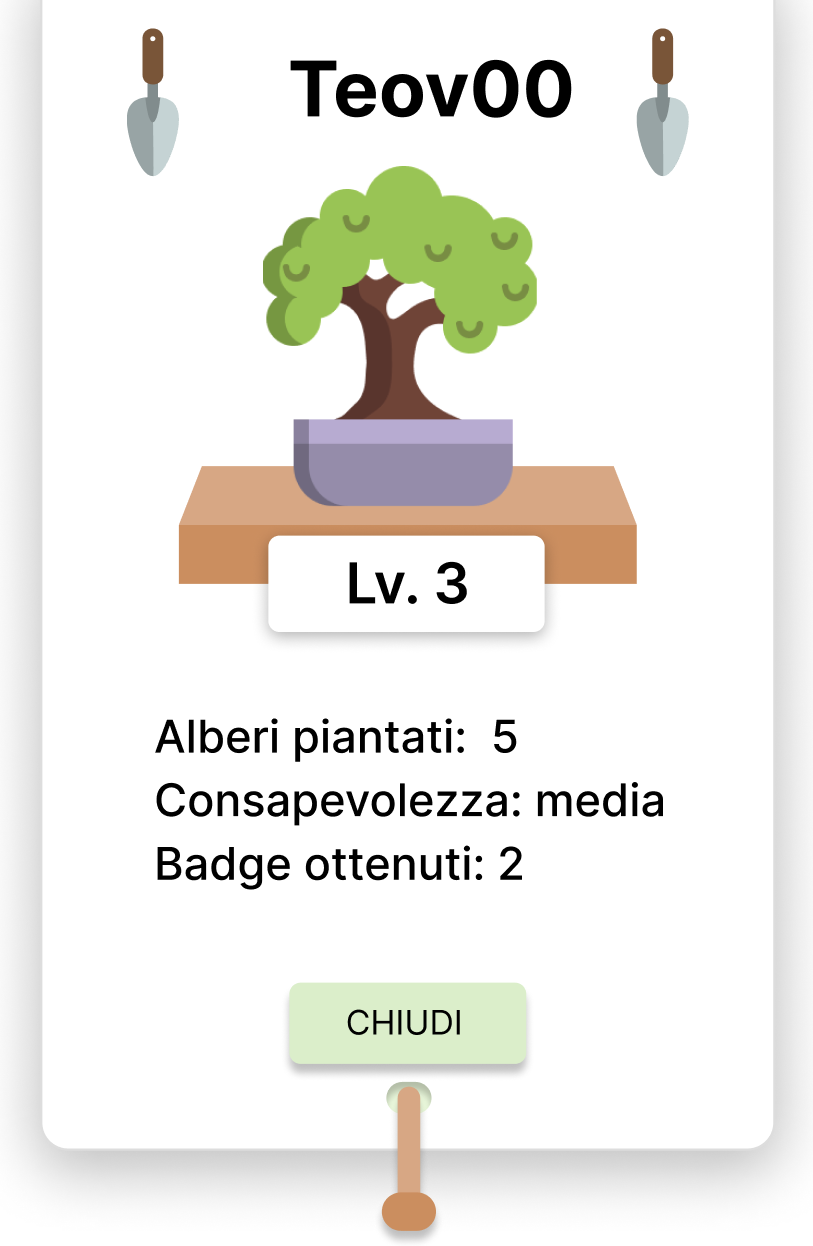
\includegraphics[width=0.30\textwidth]{img/totem/cordDetail.png}
        \label{fig:cordDetail}
    }
    \subfloat[Stile curvo]{
        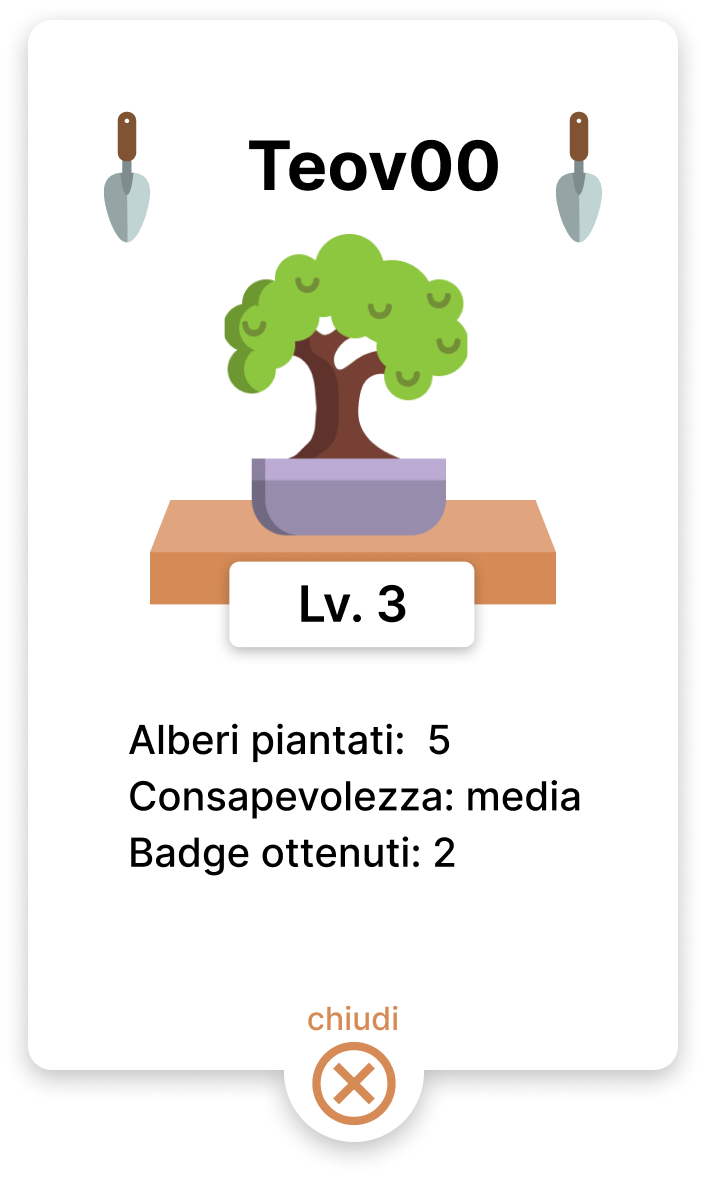
\includegraphics[width=0.28\textwidth]{img/totem/roundDetail.png}
        \label{fig:roundDetail}
    }
    \caption{Tre diversi stili per il pannello dei dettagli nel totem}
    \label{fig:detailBanner}
\end{figure}

La pagina delle statistiche (figura \ref{fig:statsPage}) mostra sei contatori (figura \ref{fig:statItem}) ciascuno per un dato disposti in una griglia di tre colonne e due righe. Il contatore è stato pensato come un cerchio colorato in modo proporzionale al valore (idea successivamente abbandonata), con all'interno un'icona rappresentativa della statistica (figura \ref{fig:statCircle}). Al tocco del singolo elemento viene mostrata una breve descrizione del dato \ref{fig:descrShowedStats}.

\begin{figure}
    \centering
    \subfloat[]{
        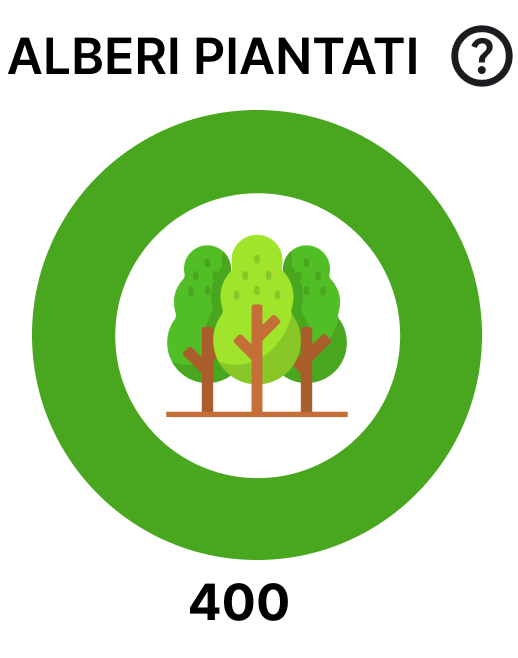
\includegraphics[width=3cm]{img/totem/plantedTreeStats.png}
        \label{fig:statCircle}
    }
    \subfloat[]{
        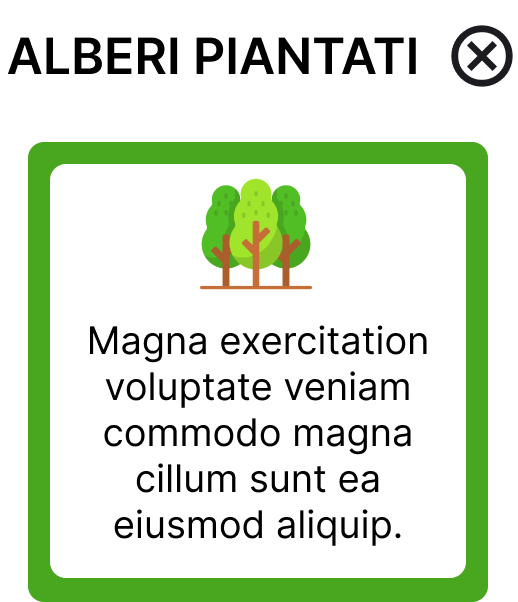
\includegraphics[width=3cm]{img/totem/plantedTreeStatsdescr.png}
        \label{fig:descrShowedStats}
    }
    \caption{Elemento contatore nella pagina statistiche}
    \label{fig:statItem}
\end{figure}

\begin{figure}
    \centering
    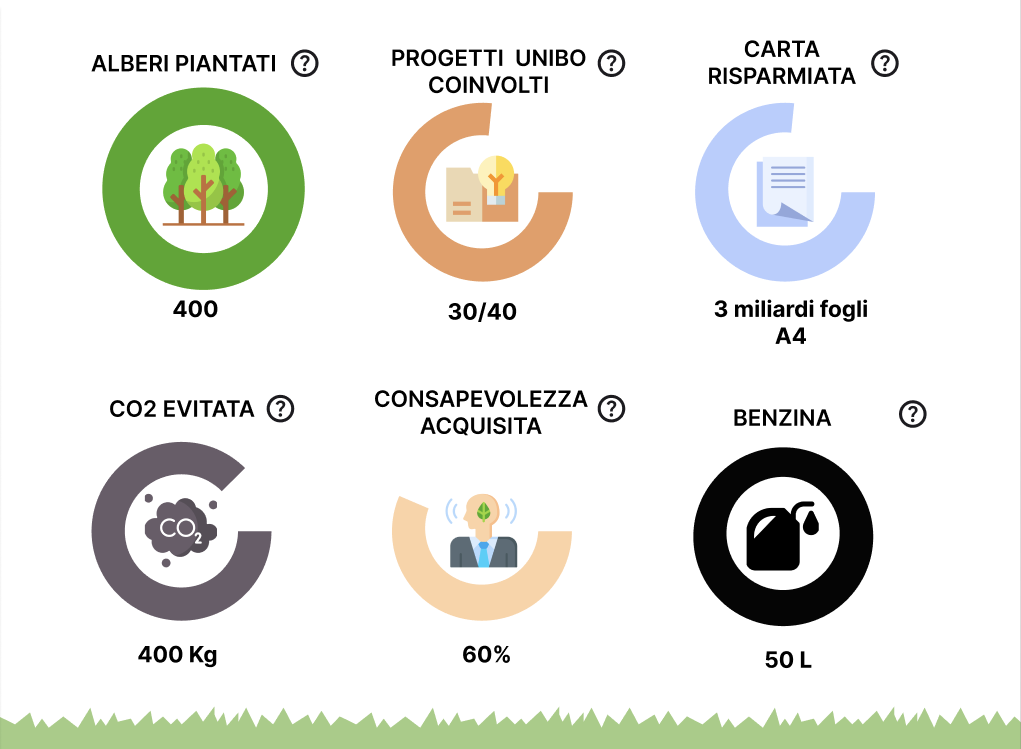
\includegraphics[width=0.8\textwidth]{img/totem/statsPage.png}
    \caption{Pagina delle statistiche}
    \label{fig:statsPage}
\end{figure}

La schermata della classifica (figura \ref{fig:chartPage}), in questa prima fase di design, è stata pensata molto semplice con una classifica, suddivisa su due colonne, degli utenti. Gli elementi della classifica indicano la posizione e il nickname dell'utente. I primi tre classificati presentano una coccarda e sono disposti come se fossero su un podio.
\begin{figure}
    \centering
    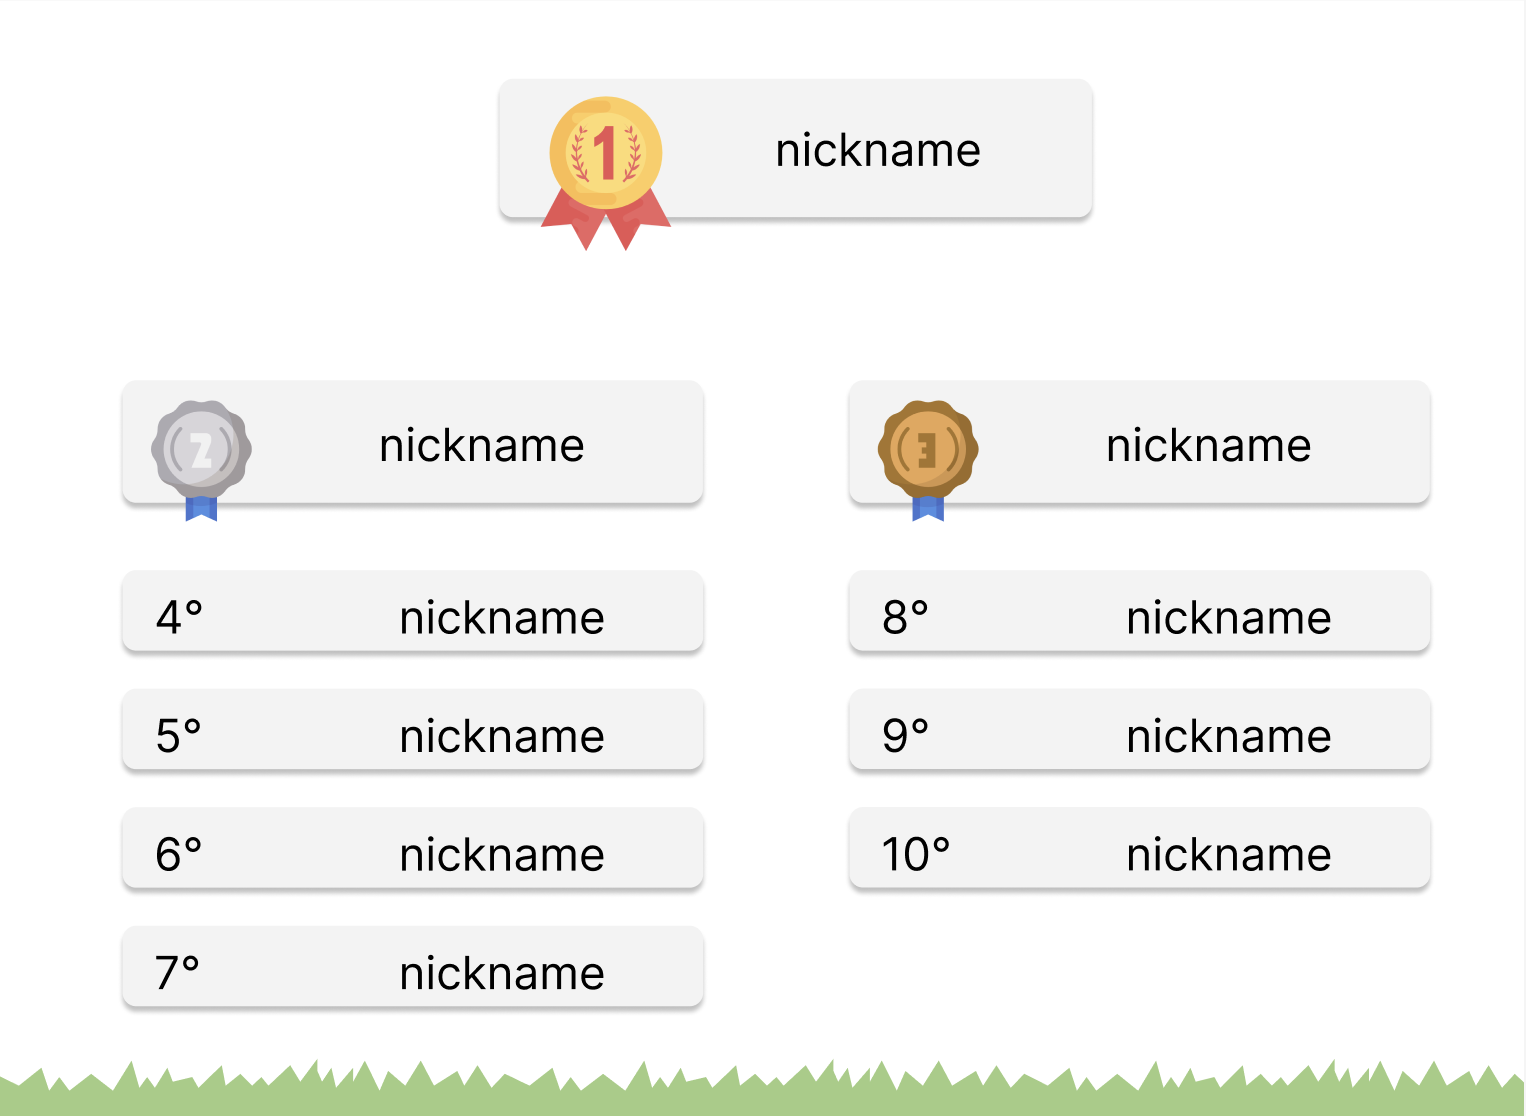
\includegraphics[width=0.8\textwidth]{img/totem/topchartPage.png}
    \caption[Classifica Top10 nel totem]{Pagina della classifica dei 10 migliori utenti}
    \label{fig:chartPage}
\end{figure}

La pagina delle informazioni nel suo primo stato embrionale, era stata concepita come una unica pagina scorrevole, simile ad una pagina web, suddivisa per sezioni ma poi è stata ripensata completamente arrivando al design in figura \ref{fig:infoPage}. Il nuovo design prevede un layout a griglia che presenta diversi \textit{tile}s (in italiano \enquote*{piastrelle}). Ciascuna \textit{tile} mostra una prima informazione riassuntiva, che può essere del testo o una immagine, e al suo tocco si espande mostrando maggiori dettagli. Con questo design l'utente può trovare, in un'unica pagina, tutti i dettagli e le informazioni riguardo al progetto con un solo sguardo e un paio di tocchi.

\begin{figure}
    \centering
    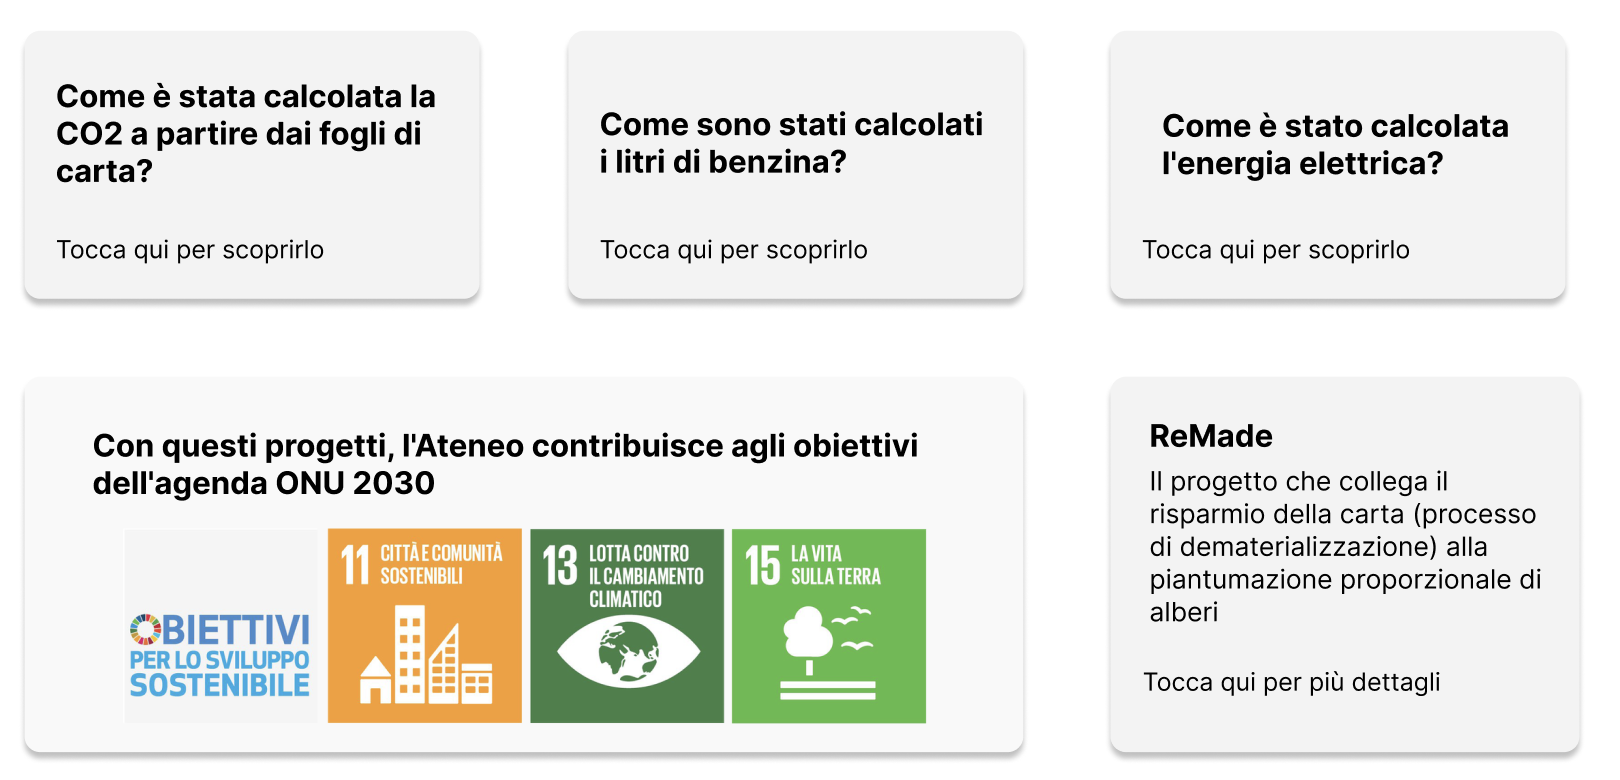
\includegraphics[width=0.8\textwidth]{img/totem/infoPage.png}
    \caption{Pagina delle informazioni con griglia di tiles}
    \label{fig:infoPage}
\end{figure}

Tutte le schermate di cui sono state sviluppate più versioni sono state poi sottoposte a un gruppo di utenti target per comprendere quale dei diversi design andasse a soddisfare al meglio le loro esigenze in termini di usabilità e grafica.

%
%
%
\newpage
\section{Tecnologie impiegate}
In questa sezione vengono presentate le tecnologie utilizzate per lo sviluppo dell'applicativo del totem e dell'applicazione mobile. Per entrambi i dispositivi si è sviluppato utilizzando il framework Flutter, per l'integrazione e gestione dei dati è stato utilizzato il servizio cloud Firebase Realtime, mentre per l'identificazione degli alberi e del totem sono stati utilizzati i codici QR.

\subsection{Figma}
Per lo sviluppo della UI e per la creazione del mockup è stato utilizzato Figma \cite{figma} che è un'applicazione web collaborativa per lo sviluppo d'interfacce utente, prototipazione interattiva e progettazione grafica.
Figma permette di testare direttamente sugli smartphone, tablet e computer i prototipi sviluppati, utilizzare plugin o creare un progetto da un template esistente. In assenza di connessione è possibile utilizzare la maggior parte delle funzionalità, escluse la collaborazione con colleghi e l'utilizzo di alcuni plugin che necessitano d'internet.
 Con questo programma inoltre è possibile manipolare e creare grafiche vettoriali (formato .svg) ed esportare lo stile di un elemento in formato CSS o per iOS e Android.

\subsection{Flutter}
Flutter \cite{flutter} è un kit di sviluppo software (\textit{Software Development Kit}, SDK) open-source che comprende diversi strumenti (\textit{DevTools}) per lo sviluppo di applicazioni multi-piattaforma con particolare attenzione all'interfaccia utente (UI, \textit{User Interface}). All'interno del SDK è contenuto il framework Flutter che utilizza il linguaggio di programmazione Dart, anch'esso sviluppato da Google, e librerie grafiche predefinite per le piattaforme Android e iOS.

Flutter, grazie a Dart, eredita il vantaggio di poter sviluppare applicazioni con interfaccia utente per diverse piattaforme e dispositivi in molta semplicità anche grazie al ricco bacino di librerie e framework che permettono di sfruttare al meglio l'architettura nativa, e nel caso di esigenze particolari, è possibile innestare codice nativo (es. Swift per iOS o Java per Android) all'interno del codice scritto in Dart. Per queste caratteristiche si è deciso di utilizzare Flutter per il totem, anche in un'ottica di futuri aggiornamenti o integrazioni con nuovi device o hardware che richiedono una determinata piattaforma; in tal caso non ci sarebbe il bisogno occorrerebbe semplicemente impostare la piattaforma target del progetto e ricompilare, senza il bisogno di riscrivere il codice sorgente con linguaggio nativo.

Il linguaggio Dart è un linguaggio di programmazione ad alto livello multi paradigma, influenzato da altri linguaggi come il C e Java, ed è ottimizzato per lo sviluppo veloce di applicazioni su qualsiasi piattaforma nativa e web.
Utilizzare il linguaggio Dart porta diversi vantaggi come la possibilità di sviluppare con un unico codice sorgente per più piattaforme, la ricerca di bug ed errori risulta semplificata e sono presenti molteplici librerie e plugin per sfruttare le funzionalità native. Di contro si ha meno controllo dell'architettura sottostante e minore accesso alle API native delle piattaforme, si possono avere prestazioni inferiori ed è possibile che, dopo la conversione in codice nativo, i framework utilizzati non siano completamente compatibili.

\subsubsection{Plugin utilizzati}
Di seguito si elencano i plugin flutter utilizzati nello sviluppo dell'applicativo del totem:
\begin{itemize}
    \item \texttt{flutter\_svg} \cite{providerPlugin}, per la visualizzazione delle immagini vettoriali utilizzate per la rappresentazione dei livelli utente e alcuni elementi grafici dell'interfaccia;
    \item \texttt{firebase\_core} \cite{firebaseCorePlugin} e \texttt{firebase\_database} \cite{firebaseDatabasePlugin}, pacchetti per poter utilizzare i servizi Firebase e quindi l'accesso al database;
    \item \texttt{barcode} \cite{barcodePlugin}, è una libreria per la generazione di codici a barre e QR;
    \item \texttt{provider} \cite{providerPlugin}, permette di utilizzare coma maggiore facilità e semplicità il widget flutter InheritedWidget che serve a propagare una informazione nell'albero dei widget.
\end{itemize}
\subsection{Firebase Realtime}
Firebase Realtime \cite{firebase} è un database non relazionale (NoSQL) memorizzato nel cloud, gestito da Google. In quanto NoSQL, i dati e le relazioni non vengono memorizzati in tabelle ma in documenti, archivi \textit{wide-column} o grafi (nodi e archi) a seconda della tipologia del database.
Firebase Realtime è di tipo documentale e quindi fa uso di documenti in formato JSON (\textit{JavaScript Object Notation}) per salvare i dati. Questo genere di memorizzazione permette maggiore flessibilità dello schema permettendo l'aggiunta o la modifica del modello dei dati (es. aggiunta o modifica di un campo). Inoltre i database NoSQL consentono una maggiore velocità e agilità di memorizzazione ed elaborazione oltre che offrire una maggiore scalabilità.
Firebase mette a disposizione anche diversi strumenti per la gestione e analisi degli accessi, permette d'installare estensioni aggiungendo funzionalità e automazioni al database e infine è possibile essere notificati a ogni aggiornamento o modifica dei dati in modo da mostrare sempre i dati più recenti all'utente.

%
\subsection{Codici QR}
Il codice QR (\textit{Quick Response}) è un tipo di codice a barre a matrice (codice 2D) sviluppato e presentato nel 1994 dalla compagnia giapponese Denso Wave che si compone di tanti piccoli quadrati neri e bianchi, chiamati moduli, disposti in una matrice \cite{qrCodeDensoWave}.
I codici QR permettono di memorizzare una quantità variabile di dati che dipende dalla tipologia di dato, dalla versione utilizzata e dal livello di correzione dell'errore. La dimensione della matrice è definita dalla versione utilizzata e anche dalla tipologia di codice QR (Modello 1 o 2, \textit{Micro QR Code}, \textit{rMQR Code}, \textit{SQRC}, Frame QR).

La versione più comune di \textit{QR code} è di tipo \textit{Model 1 o 2} di livello 3, presenta 29x29 moduli ed è in grado di memorizzare fino ad un massimo di 77 caratteri alfanumerici con la correzione dell'errore del 7\% circa.

\section{Strumenti di sviluppo}
\subsection{Git}
Git \cite{gitSite} è un \textit{Version Control System} VCS cioè un sistema di controllo delle versioni dei file. I cambiamenti di uno o più file nel tempo vengono memorizzati e questo permette di mantenere una cronologia dei cambiamenti e di ripristinare una versione precedente di file, cartelle o interi progetti. Esistono diverse tipologie di VCS: locale, centralizzato o distribuito.
Rispetto ai tradizionali VCS, Git non memorizza le differenze dei file (\textit{delta-based version control}) ma memorizza una istantanea di come appaiono i file nel \textit{filesystem} nell'istante in cui si effettua un salvataggio di versione (\textit{commit}). Git considera i suoi dati più come a un flusso d'istantanee del progetto che viene tracciato. Git possiede un sistema di branching/merging avanzati e di gestione dei conflitti che sono stati utilizzati durante lo sviluppo delle funzionalità e schermate del totem.

\subsection{Visual Studio Code}
Visual Studio Code \cite{vsCodeSite} è un editor di codice sorgente, sviluppato da Microsoft per Windows, Mac e Linux. Prevede diverse funzionalità utili per la scrittura di codice come la previsione e suggerimento di codice (IntelliSense) e gli strumenti di segnalazione e correzione degli errori, che i comuni editor di testo non possiedono.
Può essere utilizzato con la maggior parte dei linguaggi di programmazione (es. C, Java, PHP) ed è possibile aggiungerne di nuovi ed estendere le sue capacità attraverso dei \textit{plugin} scaricabili direttamente all'interno di Visual Studio Code.
Viste le qualità di questo editor e al suo utilizzo pregresso si è deciso di utilizzarlo per lo sviluppo di questo progetto con l'integrazione del \textit{plugin} ufficiale di Flutter che aggiunge ulteriori strumenti di analisi e \textit{debug}.